%\documentclass{sig-alternate-05-2015}
\documentclass{llncs}
\usepackage{makeidx}
\usepackage{tabularx,colortbl}
\usepackage[dvipsnames]{xcolor}
\usepackage{flushend}
\usepackage{cite}
\usepackage{amsmath}
%\usepackage{amsthm}
\usepackage{amssymb}
\usepackage{epsfig}
\usepackage{stmaryrd}
\usepackage{url}
\usepackage{multirow}
\usepackage{latexsym}
\usepackage{graphics}
\usepackage{graphicx}
\usepackage{enumitem}
\usepackage{comment}
\usepackage{longtable}
\usepackage{supertabular}
\usepackage{times}
\usepackage{listings}
\usepackage{subfigure}
\usepackage{color}
\usepackage{balance}
\usepackage{xspace}
\usepackage[ruled, vlined, linesnumbered]{algorithm2e}
\usepackage[autostyle]{csquotes}
\usepackage[]{algorithm2e}



%\theoremstyle{Definition}
%\newtheorem{definition}{Definition}
%%%
%\theoremstyle{Theorem}
%\newtheorem{theorem}{Theorem}


%\newcommand{\definition}{\noindent \textbf{Definition} \citation{}}
%\newcommand{\theorem}{\noindent \textbf{Theorem} \citation{}}
%\newcommand{\lemma}{\noindent \textbf{Lemma} \citation{}}

%\newdef{lemma}{Lemma}
%\newdef{definition}{Definition}
%\newdef{theorem}{Theorem}
%\newdef{corollary}{Corollary}
%\newdef{note}{Note}
%\newdef{axiom}{Axiom}
\newcommand{\mkeyword}[1]{\mbox{\texttt{#1}}}
\DeclareMathOperator{\kuop}{uop}
\DeclareMathOperator{\kbop}{bop}
\DeclareMathOperator{\kite}{ite}
\DeclareMathOperator{\kpre}{pre}
\DeclareMathOperator{\dom}{dom}
\DeclareMathOperator{\ktrue}{true}
\DeclareMathOperator{\kfalse}{false}
\DeclareMathOperator{\kselect}{select}
\DeclareMathOperator{\ran}{range}
\newcommand{\lbb}{[\![}
\newcommand{\rbb}{]\!]}
\newcommand{\expr}{\phi}
\newcommand{\exprS}{\Phi}
\newcommand{\mats}[1]{\textcolor{red}{#1}}
\newcommand{\janet}[1]{\textcolor{blue}{#1}}
\newcommand{\darren}[1]{\textcolor{green}{#1}}
\newcommand{\danielle}[1]{\textcolor{orange}{#1}}

\sloppypar



\begin{document}

\definecolor{gold}{rgb}{0.90,.66,0}
\definecolor{dgreen}{rgb}{0,0.6,0}
\newcommand{\stateequiv}{\equiv_{s}}
\newcommand{\traceequiv}{\equiv_{\sigma}}
\newcommand{\ta}{\text{TA}}
\newcommand{\cta}{\text{TA$_{C}$}}
\newcommand{\tta}{\text{TA$_{T}$}}
\newcommand{\ucalg}{\texttt{\small{IVC\_UC}}}
\newcommand{\ucbfalg}{\texttt{\small{IVC\_UCBF}}}


\title{Safety Annex for the Architecture Analysis and Design Language}
%
\author{Danielle Stewart\inst{1}
\and Jing (Janet) Liu\inst{2}
\and Michael W. Whalen\inst{1}
\and Darren Cofer\inst{2}
\and Mats Heimdahl\inst{2}
\and Michael Peterson\inst{3}}
\institute{University of Minnesota\\Department of Computer
Science and Engineering\\
\email{dkstewar, whalen, heimdahl}@cs.umn.edu
\and
Rockwell Collins\\
Advanced Technology Center\\
\email{Jing.Liu, Darren.Cofer}@rockwellcollins.com
\and
Rockwell Collins\\
Commercial Systems Flight Controls Safety Engineering\\
\email{Michael.Peterson}@rockwellcollins.com
}
\maketitle

\begin{abstract}
%Mats' abstract
Model-based development techniques are increasingly being used in the development of critical systems software. Leveraging the artifacts from model based development in the safety analysis process would be highly desirable to provide accurate analysis and enable cost savings. In particular, the architectural and behavioral models provide rich information on the system's operation. In this paper we describe an extension (an Annex) to the Architecture Analysis and Design Language (AADL) developed to allow a rich modeling of a system under failure conditions. This \emph{Safety Annex} allows the independent modeling of component failure modes and allows safety engineers to weave various types of faults into the nominal system model. The accompanying tool support allows investigation of the \emph{implicit} propagation of failures from their source to their effect on top level safety properties as well as the modeling of \emph{explicit} failure propagation that is not captured through the behavioral models, e.g., failures correlated due to the physical structure of the system. We describe the Safety Annex, illustrate its use with a representative example, and discuss and demonstrate the tool support enabling an analyst to investigate the system behavior under various failure conditions.	
	
%This paper describes a new methodology with tool support for model-based safety analysis. It is implemented as a {\em Safety Annex} for the Architecture Analysis and Design Language (AADL). The Safety Annex provides the ability to describe faults and faulty component behaviors in AADL models. In contrast to previous AADL-based approaches, the Safety Annex leverages a formal description of the nominal system behavior to propagate faults in the system. This approach ensures consistency with the rest of the system development process and simplifies the work of safety engineers. The language for describing faults is extensible and allows safety engineers to weave various types of faults into the nominal system model. The Safety Annex supports the injection of faults into component level outputs, and the resulting behavior of the system can be analyzed using model checking through the Assume-Guarantee Reasoning Environment (AGREE).

%System safety assessment is a crucial process in the development of complex airborne systems to show that the relevant safety requirements are met. Acquiring the required knowledge about how the software functions are intended to work in such systems has shown in practice a very involved and time consuming task. Existing approaches that annotate the system architecture model with failure modes and fault propagations help safety analysts better communicate with system designers and address the complexity of the system. However, knowledge on how the faults propagate through the components still needs to be acquired before such information can be captured in the model. Nor do the models capture analyzable behaviors. The methodology described in this paper enables safety analysts to specify faults and faulty behaviors at individual components (using the Safety Annex for the Architecture Analysis and Design Language (AADL)). The provided tool support auto weaves the faults into the nominal system model provided by system designers. No additional effort is needed to specify fault propagations as the faulty behavior propagates in the nominal system model the same as the normal behavior. The behavior of the system in the presence of faults are verified using model checking through Assume Guarantee Reasoning Environment (AGREE), and the effects of any triggered fault are manifested in the formal analysis results.

%System safety assessment is a crucial process in the development of complex airborne systems to show that the relevant safety requirements are met. Acquiring the required knowledge about how the software functions are intended to work in such systems has shown in practice a very involved and time consuming task. Existing approaches that annotate the system architecture model with failure modes and fault propagations help safety analysts better communicate with system designers and address the complexity of the system. However, knowledge on how the faults propagate through the components still needs to be acquired by safety analysts before such information can be captured in the model. Acquiring the information on fault propagation is still a manual effort. The methodology described in this paper enables safety analysts to specify faults and faulty behaviors at individual components (using the Safety Annex for the Architecture Analysis and Design Language (AADL)). The provided tool support auto weaves the faults into the nominal system model provided by system designers. No additional effort is needed to specify fault propagations as the faulty behavior propagates in the nominal system model the same as the normal behavior. The behavior of the system in the presence of faults are verified using model checking through Assume Guarantee Reasoning Environment (AGREE), and the effects of any triggered fault are manifested in the formal analysis results.

\end{abstract}

\keywords{Model-based systems engineering, fault analysis, safety engineering}

\section{Introduction}

System safety analysis techniques are well established and are a required activity in the development of commercial aircraft and safety-critical ground systems. However, these techniques are based on informal system descriptions that are separate from the actual system design artifacts, and are highly dependent on the skill and intuition of a safety analyst. The lack of precise models of the system architecture and its failure modes often forces safety analysts to devote significant effort to gathering architectural details about the system behavior from multiple sources and embedding this information in safety artifacts, such as fault trees.

While model-based development (MBD) methods are widely used in the aerospace industry, they are generally disconnected from the safety analysis process itself. Formal model-based systems engineering (MBSE) methods and tools~\cite{QFCS15:backes,hilt2013,NFM2012:CoGaMiWhLaLu,DBLP:journals/scp/CimattiT15,Pajic2012,DBLP:conf/adaEurope/SokolskyLC09} now permit system-level requirements to be specified and analyzed early in the development process. These tools can also be used to perform safety analysis based on the system architecture and initial functional decomposition. Design models from which aircraft systems are developed can be integrated into the safety analysis process to help guarantee accurate and consistent results. This integration is especially important as the amount of safety-critical hardware and software in domains such as aerospace, automotive, and medical devices has dramatically increased due to desire for greater autonomy, capability, and connectedness.

Architecture description languages, such as SysML~\cite{SysML} and the Architecture Analysis and Design Language (AADL)~\cite{AADL} are appropriate for capturing system safety information.  There are several tools that currently support reasoning about faults in architecture description languages, such as the AADL error annex~\cite{Larson:2013:IAE:2527269.2527271} and HiP-HOPS for EAST-ADL~\cite{CHEN201391}.  However, these approaches primarily use {\em qualitative} reasoning, in which faults are enumerated and their propagations through system components must be explicitly described.  Given many possible faults, these propagation relationships become complex and it is also difficult to describe temporal properties of faults that evolve over time (e.g., leaky valve or slow divergence of sensor values).

In earlier work, University of Minnesota and Rockwell Collins developed and demonstrated an approach to model-based safety analysis (MBSA) \cite {Joshi05:Dasc,Joshi05:SafeComp,NasaRep:MBSA-Aug05} using the Simulink notation \cite{MathWorks}.  In this approach, a behavioral model of (sometimes simplified) system dynamics was used to reason about the effect of faults.  We believe that this approach allows a natural and implicit notion of fault propagation through the changes in pressure, mode, etc. that describe the system's behavior.  Unlike qualitative approaches, this approach allows uniform reasoning about system functionality and failure behavior, and can describe complex temporal fault behaviors.  On the other hand, Simulink is not an architecture description language, and several system engineering aspects, such as hardware devices and non-functional aspects cannot be easily captured in models.

\iffalse
Over the last five years, several research groups have focused on formal reasoning at the system architecture level, resulting in MBSE tools that incorporate assume-guarantee compositional reasoning techniques~\cite{Trento and Rockwell and UMN}.  These tools allow behavioral reasoning about complex system models, but with substantially greater scalability than previous approaches.
\fi

This paper describes our initial work towards a behavioral approach to MBSA using AADL.  Using assume-guarantee compositional reasoning techniques, we hope to support system safety objectives of ARP4754A and ARP4761.  To make these capabilities accessible to practicing safety engineers, it is necessary to extend modeling notations to better describe failure conditions, interactions, and mitigations, and provide improvements to compositional reasoning approaches focused on the specific needs of system safety analysis.  These extensions involve creating models of fault effects and weaving them into the analysis process.  To a large extent, our work has been an adaptation of the work of Joshi et. al to the AADL modeling language.

To evaluate the effectiveness and practicality of our approach, we developed an architectural model of the Wheel Braking System model in SAE AIR6110.  Starting from a reference AADL model constructed by the SEI instrumented with qualitative safety analysis information~\cite{SEI:AADL}, we added behavioral contracts to the model.  In so doing, we determine that there are errors related to (manually constructed) propagations across components, and also an architecture that contains single points of failure.  We use our analyses to find and fix these errors.

The rest of the paper is organized as follows...





\section{Preliminaries}
\label{sec:prelims}
One of our goals is to transition the tools we have developed into use by the safety engineers who perform safety assessment of avionics products. Therefore, we need to understand how the tools and the models will fit into the existing safety assessment and certification process.
ARP4754A, the Guidelines for Development of Civil Aircraft and Systems~\cite{SAE:ARP4754A}, provides guidance on applying development assurance at each hierarchical level throughout the development life cycle of highly-integrated/complex aircraft systems. It has been recognized by the Federal Aviation Administration (FAA) as an acceptable method to establish the assurance process. The safety assessment process is a starting point at each hierarchical level of the development life cycle and is tightly coupled with the system development and verification processes. It is used to show compliance with certification requirements and for meeting a company's internal safety standards. 

ARP4761, the Guidelines and Methods for Conducting Safety Assessment Process on Civil Airborne Systems and Equipment~\cite{SAE:ARP4761},  identifies a systematic means to show compliance. Among the industry accepted safety assessment processes are Preliminary System Safety Assessment (PSSA) and System Safety Assessment (SSA). PSSA evaluates the system design and defines safety requirements. SSA evaluates the implemented system to show that safety requirements defined in the PSSA are in fact satisfied.

A prerequisite of performing the safety assessment is understanding how the system is intended to work, primarily focusing on the integrity of the outputs and the availability of the system. The safety engineers then use the acquired understanding to conduct safety analysis, construct safety analysis artifacts, and compare the results with established safety objectives and requirements.
Typically equipped with the domain knowledge about the system, but not detailed knowledge of how the software applications are designed, practicing safety engineers find it a time consuming and involved process to acquire the knowledge about the behavior of the software applications hosted in a system and its impact on the overall system behavior.
Industry practitioners have come to realize the benefits of using models in the safety assessment process, and a revision of the ARP4761 to include Model Based Safety Analysis (MBSA) is under way.
Figure~\ref{fig:proposed_safety_process} presents our proposed use of a single unified model to support both system design and safety analysis. It describes both system design and safety-relevant information 
that are kept distinguishable and yet are able to interact with each other. The shared model maintains a living model that captures the current state of the system design as it moves through the development lifecycle, allowing all participants of the ARP4754A process to be able to communicate and review the system design. Safety analysis artifacts can be generated directly from the model, 
providing
the capability to more accurately analyze complex systems.

\begin{figure}[t!]
	\vspace{-0.45in}
	\centering
	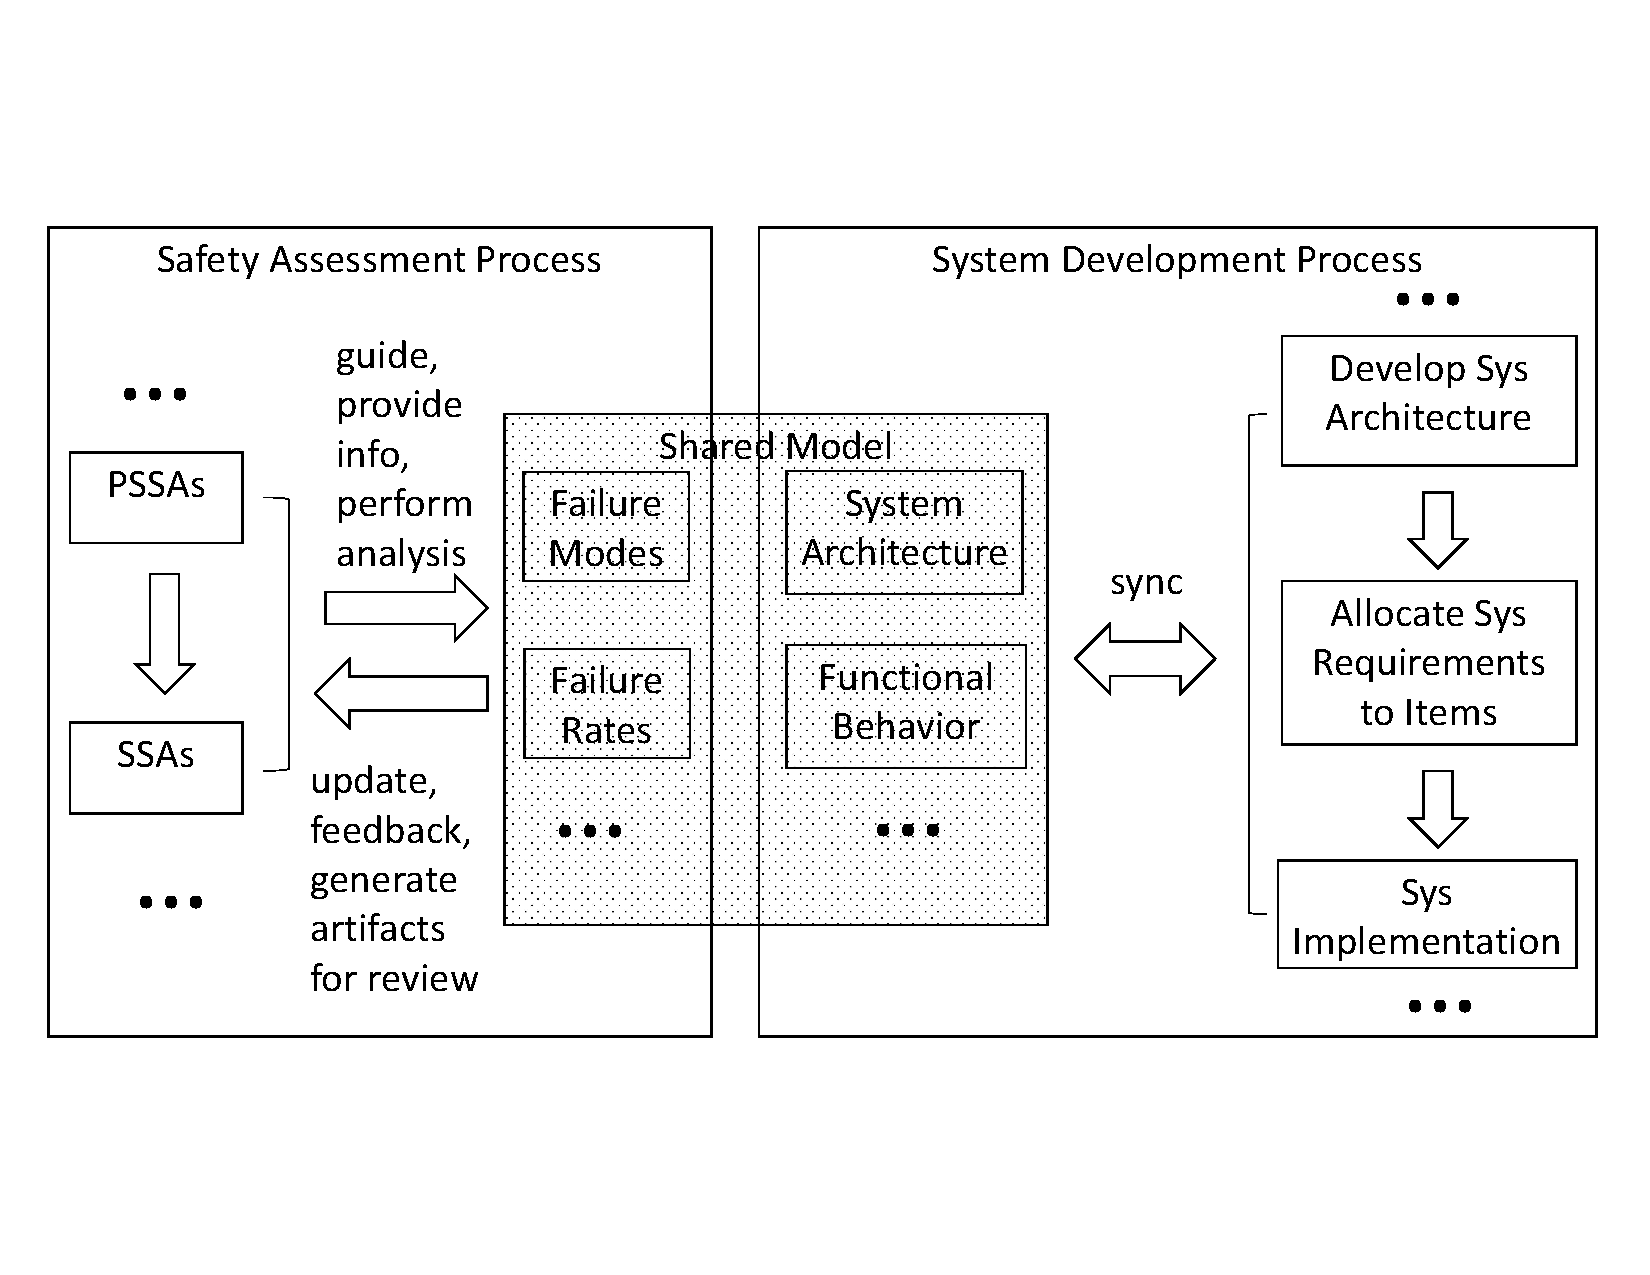
\includegraphics[trim=0 9 0 5,clip,width=0.85\textwidth]{images/safety_process.pdf}
	\vspace{-0.45in}
	\caption{Use of the Shared System/Safety Model in the ARP4754A Safety Assessment Process}
	\label{fig:proposed_safety_process}
\end{figure}

\subsection{Modeling Language for System Design}
\label{subsec:aadl-agree}
%Talk about AADL, AGREE, and why safety annex
%Pull AADL/AGREE background from previous papers to support points in the safety process
%Following the motivation/discussion in the process subsection, talk about why we choose to extend AGREE in safety annex, instead of using a separate safety model, or a semi-separate safety model like EMV2.
The Architectural Analysis and Design Language (AADL)~\cite{FeilerModelBasedEngineering2012} is an SAE International standard~\cite{AADL_Standard} that defines a language and provides a unifying framework for describing the system architecture for ``performance-critical, embedded, real-time systems''~\cite{AADL_Standard}. An AADL model describes a system in terms of a hierarchy of components and their interconnections, where each component can either represent a logical entity (e.g., application software functions, data) or a physical entity (e.g., buses, processors). An AADL model can be associated with properties and be extended with language annexes to provide a richer set of modeling elements for various system design and analysis needs (e.g., performance-related characteristics, configuration settings, dynamic behaviors). The language semantics supports formal analysis tools that allow for early phase error/fault detection.

The Assume Guarantee Reasoning
Environment (AGREE)~\cite{NFM2012:CoGaMiWhLaLu} implements as an AADL annex and annotates AADL components with formal behavioral contracts. Each component's contracts can include assumptions and guarantees about the component's inputs and outputs respectively, as well as predicates on how the state of the component can evolve over time.

AGREE translates an AADL model and the behavioral contracts into Lustre~\cite{Halbwachs91:IEEE} and then query a user-selected
model checker to conduct the back-end verification. The verification is performed compositionally along the architecture hierarchy such that verification at a higher level is only using the components and their behavioral contracts from its immediate lower level. This allows the verification to scale for the design of large and complex systems. 

\begin{comment}
This paper should define how your team of authors see the interaction between "functions" and "system".  
Here is how I see the interaction / relationship:
(a) Aircraft Functions are the highest level
(b) Aircraft Functions are comprised of one or more System
(c) Each System performs one or more System Function
(d) Each System is comprised of one or more LRUs (a.k.a. "items")
\end{comment}

AADL with the AGREE extension serves as a good candidate as the modeling language for describing the system design aspects of a shared system design and safety analysis model. Our prior work~\cite{Stewart17:IMBSA} adds the initial failure effect modeling capability to this language and tool set. However, the following goals are yet to be achieved before the combined language and tool set can be used to satisfy system safety objectives of ARP4754A~\cite{SAE:ARP4754A} and ARP4761~\cite{SAE:ARP4761}:

\begin{enumerate}
	\item Being able to provide a comprehensive, qualitative description of the causal relationship between basic events and system level safety requirements.
	\item Being able to provide an accurate, quantitative description of the contribution relationship between failure rates of the fault tree basic events and numerical probability requirements at the system level.
\end{enumerate}

The remainder of the paper describes our approach towards both of the goals.





\subsection{Example}
\label{subsec:comparison_with_EMV2}

The AADL language has previously been extended to provide some fault modeling and analysis capabilities using its Error Model Annex, Version 2 (EMV2)~\cite{EMV2}.  EMV2 focuses on injection and propagation of discrete faults for generation of fault trees, rather than on analysis of system behavior in the presence of faults. 
To illustrate some of the key differences between our approach and the EMV2 approach, Figure~\ref{fig:comparison_with_EMV2} shows a simplified example based on an aircraft Wheel Brake System (WBS). The WBS model is described in greater detail in ~\cite{Stewart17:IMBSA} and in Section \ref{sec:case_study}. The code fragments in the figure extracted from EMV2, AGREE, and the Safety Annex do not represent the complete code.

In our simplified WBS system, the physical signal from the Pedal component in detected by the Sensor, and the pedal position value is passed to the Braking System Control Unit (BSCU) components.  The BSCU generates a pressure command to the Valve component which applies hydraulic brake pressure to the Wheels. In this example, we use the general term ``fault'' to denote all component errors, hardware failures, and system faults captured by both approaches.

In the EMV2 approach (top half of Figure~\ref{fig:comparison_with_EMV2}), all faults must be explicitly propagated through each component (by applying fault types on each of the output ports) in order for a component to have an impact on the rest of the system. In the example, the ``NoService'' fault is explicitly allowed by the EMV2 declarations to propagate through all of the components.  These fault types are essentially tokens that do not capture any analyzable behavior.  At the system level, analysis tools supporting the EMV2 annex can aggregate the fault flow and propagation information from different components to compose an overall fault flow diagram or fault tree.

In the Safety Annex approach (bottom half of Figure~\ref{fig:comparison_with_EMV2}), faults are captured as faulty behaviors that augment the system behavioral model in AGREE contracts.  When a fault is triggered, the output behavior of the Sensor component is modified, in this case resulting a ``stuck at zero'' error. The behavior of the BSCU receives a zero input and proceeds as if the pedal has not been pressed. This will cause the top level system contract to fail: {\em pedal pressed implies brake pressure output is positive}. No explicit fault propagation is necessary since the faulty behavior itself propagates through the system just as in the nominal system model. The effects of any triggered fault are manifested through analysis of the AGREE contracts. 

\begin{figure}[t]
	\vspace{-0.19in}
	\centering
	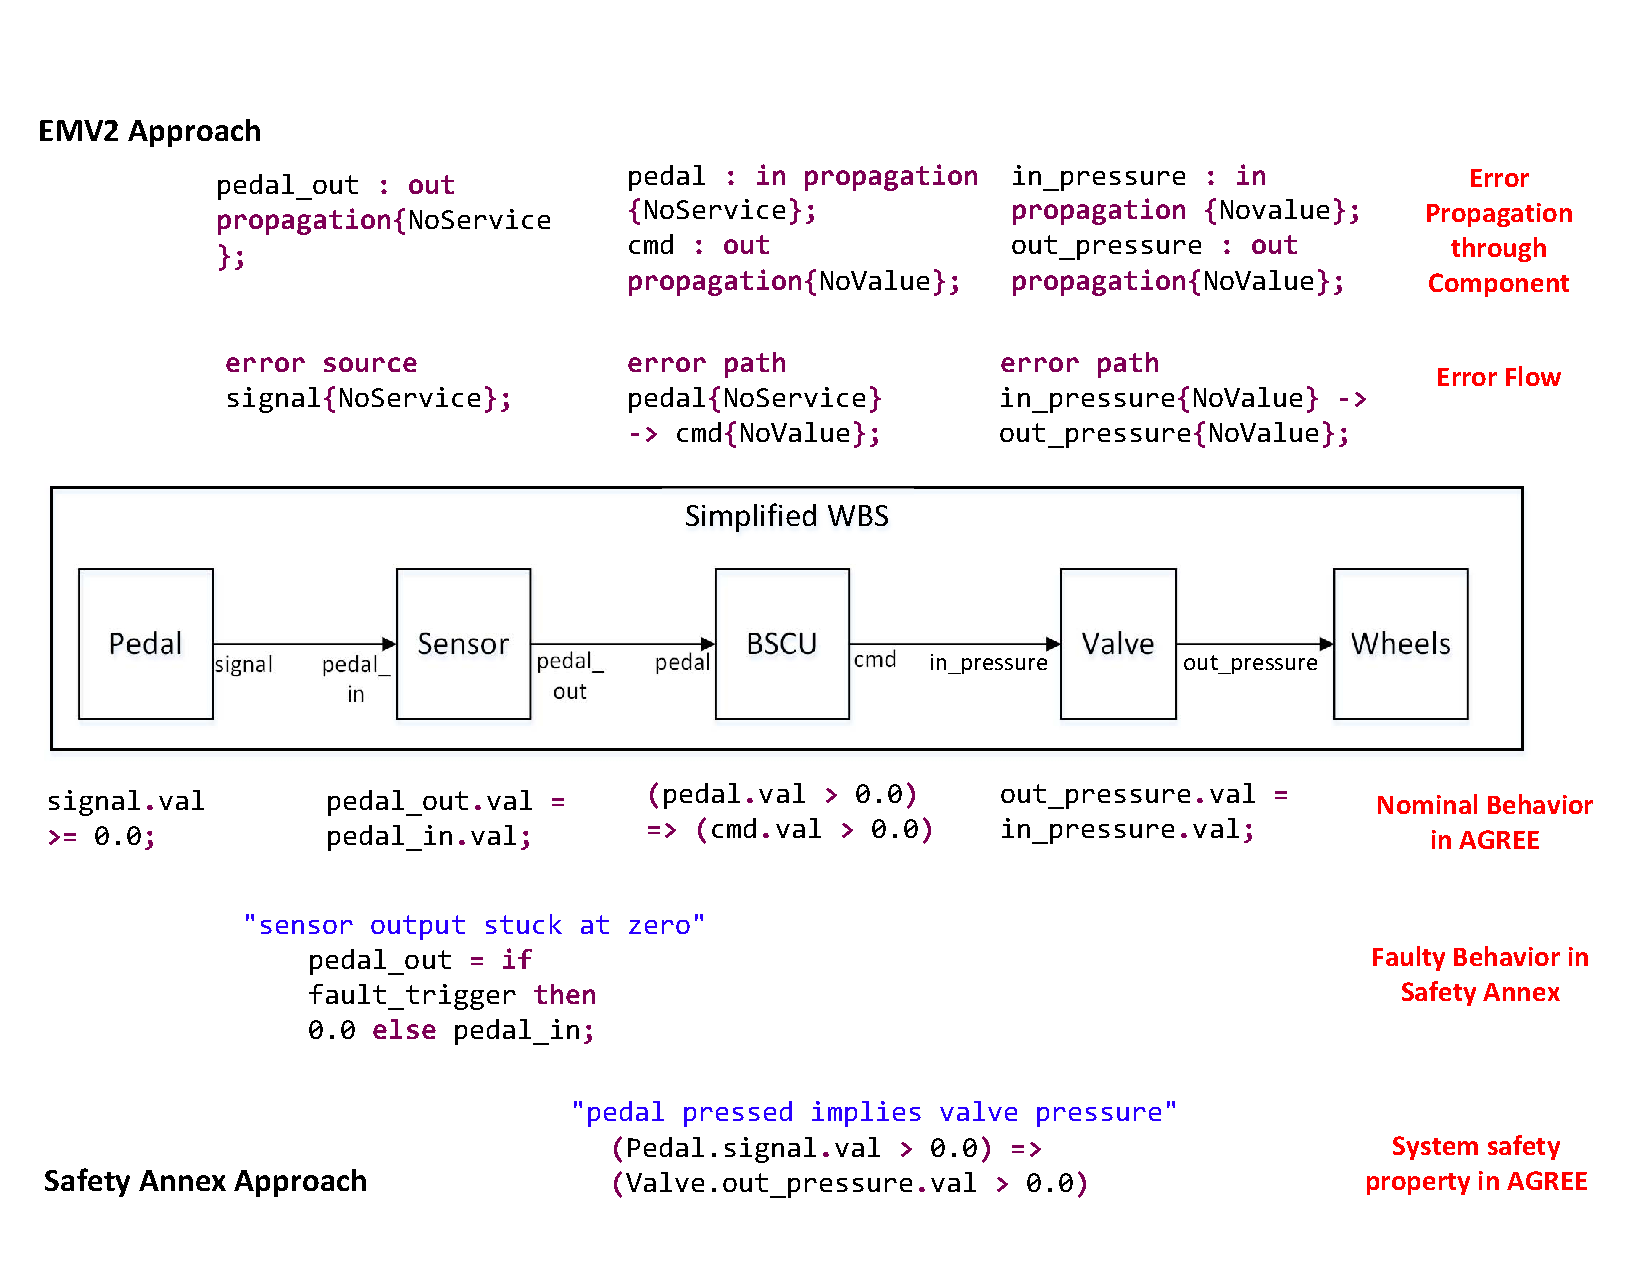
\includegraphics[trim=0 9 0 5,clip,width=\textwidth]{images/Comparison_with_EMV2.pdf}
	%\vspace{0.4in}
	\caption{Differences between Safety Annex and EMV2}
	\label{fig:comparison_with_EMV2}
\end{figure} 
 









% \section{Motivating Example}
\label{sec:case_study} 

\subsubsection{Wheel Brake System}
In order to demonstrate the fault modeling capabilities of the Safety Annex in Section~\ref{sec:fault_modeling} and provide examples of how to use the Safety Annex to perform fault modelling and analysis, we describe a model of a Wheel Brake System (WBS) of an aircraft. 

The Wheel Brake System (WBS) described in AIR6110~\cite{AIR6110} is a well-known example that has been used as a case study for safety analysis, formal verification, and contract based design~\cite{DBLP:conf/cav/BozzanoCPJKPRT15, 10.1007/978-3-319-11936-6-7, CAV2015:BoCiGrMa, Joshi05:SafeComp}. The preliminary work for the safety annex used a simplified model of the WBS~\cite{Stewart17:IMBSA}. In order to demonstrate a complex fault modeling process, we constructed a functionally and structurally equivalent AADL version of one of the most complex WBS NuSMV/xSAP models (arch4wbs) described in~\cite{DBLP:conf/cav/BozzanoCPJKPRT15}.    

\begin{figure}[h!]
	\centering
	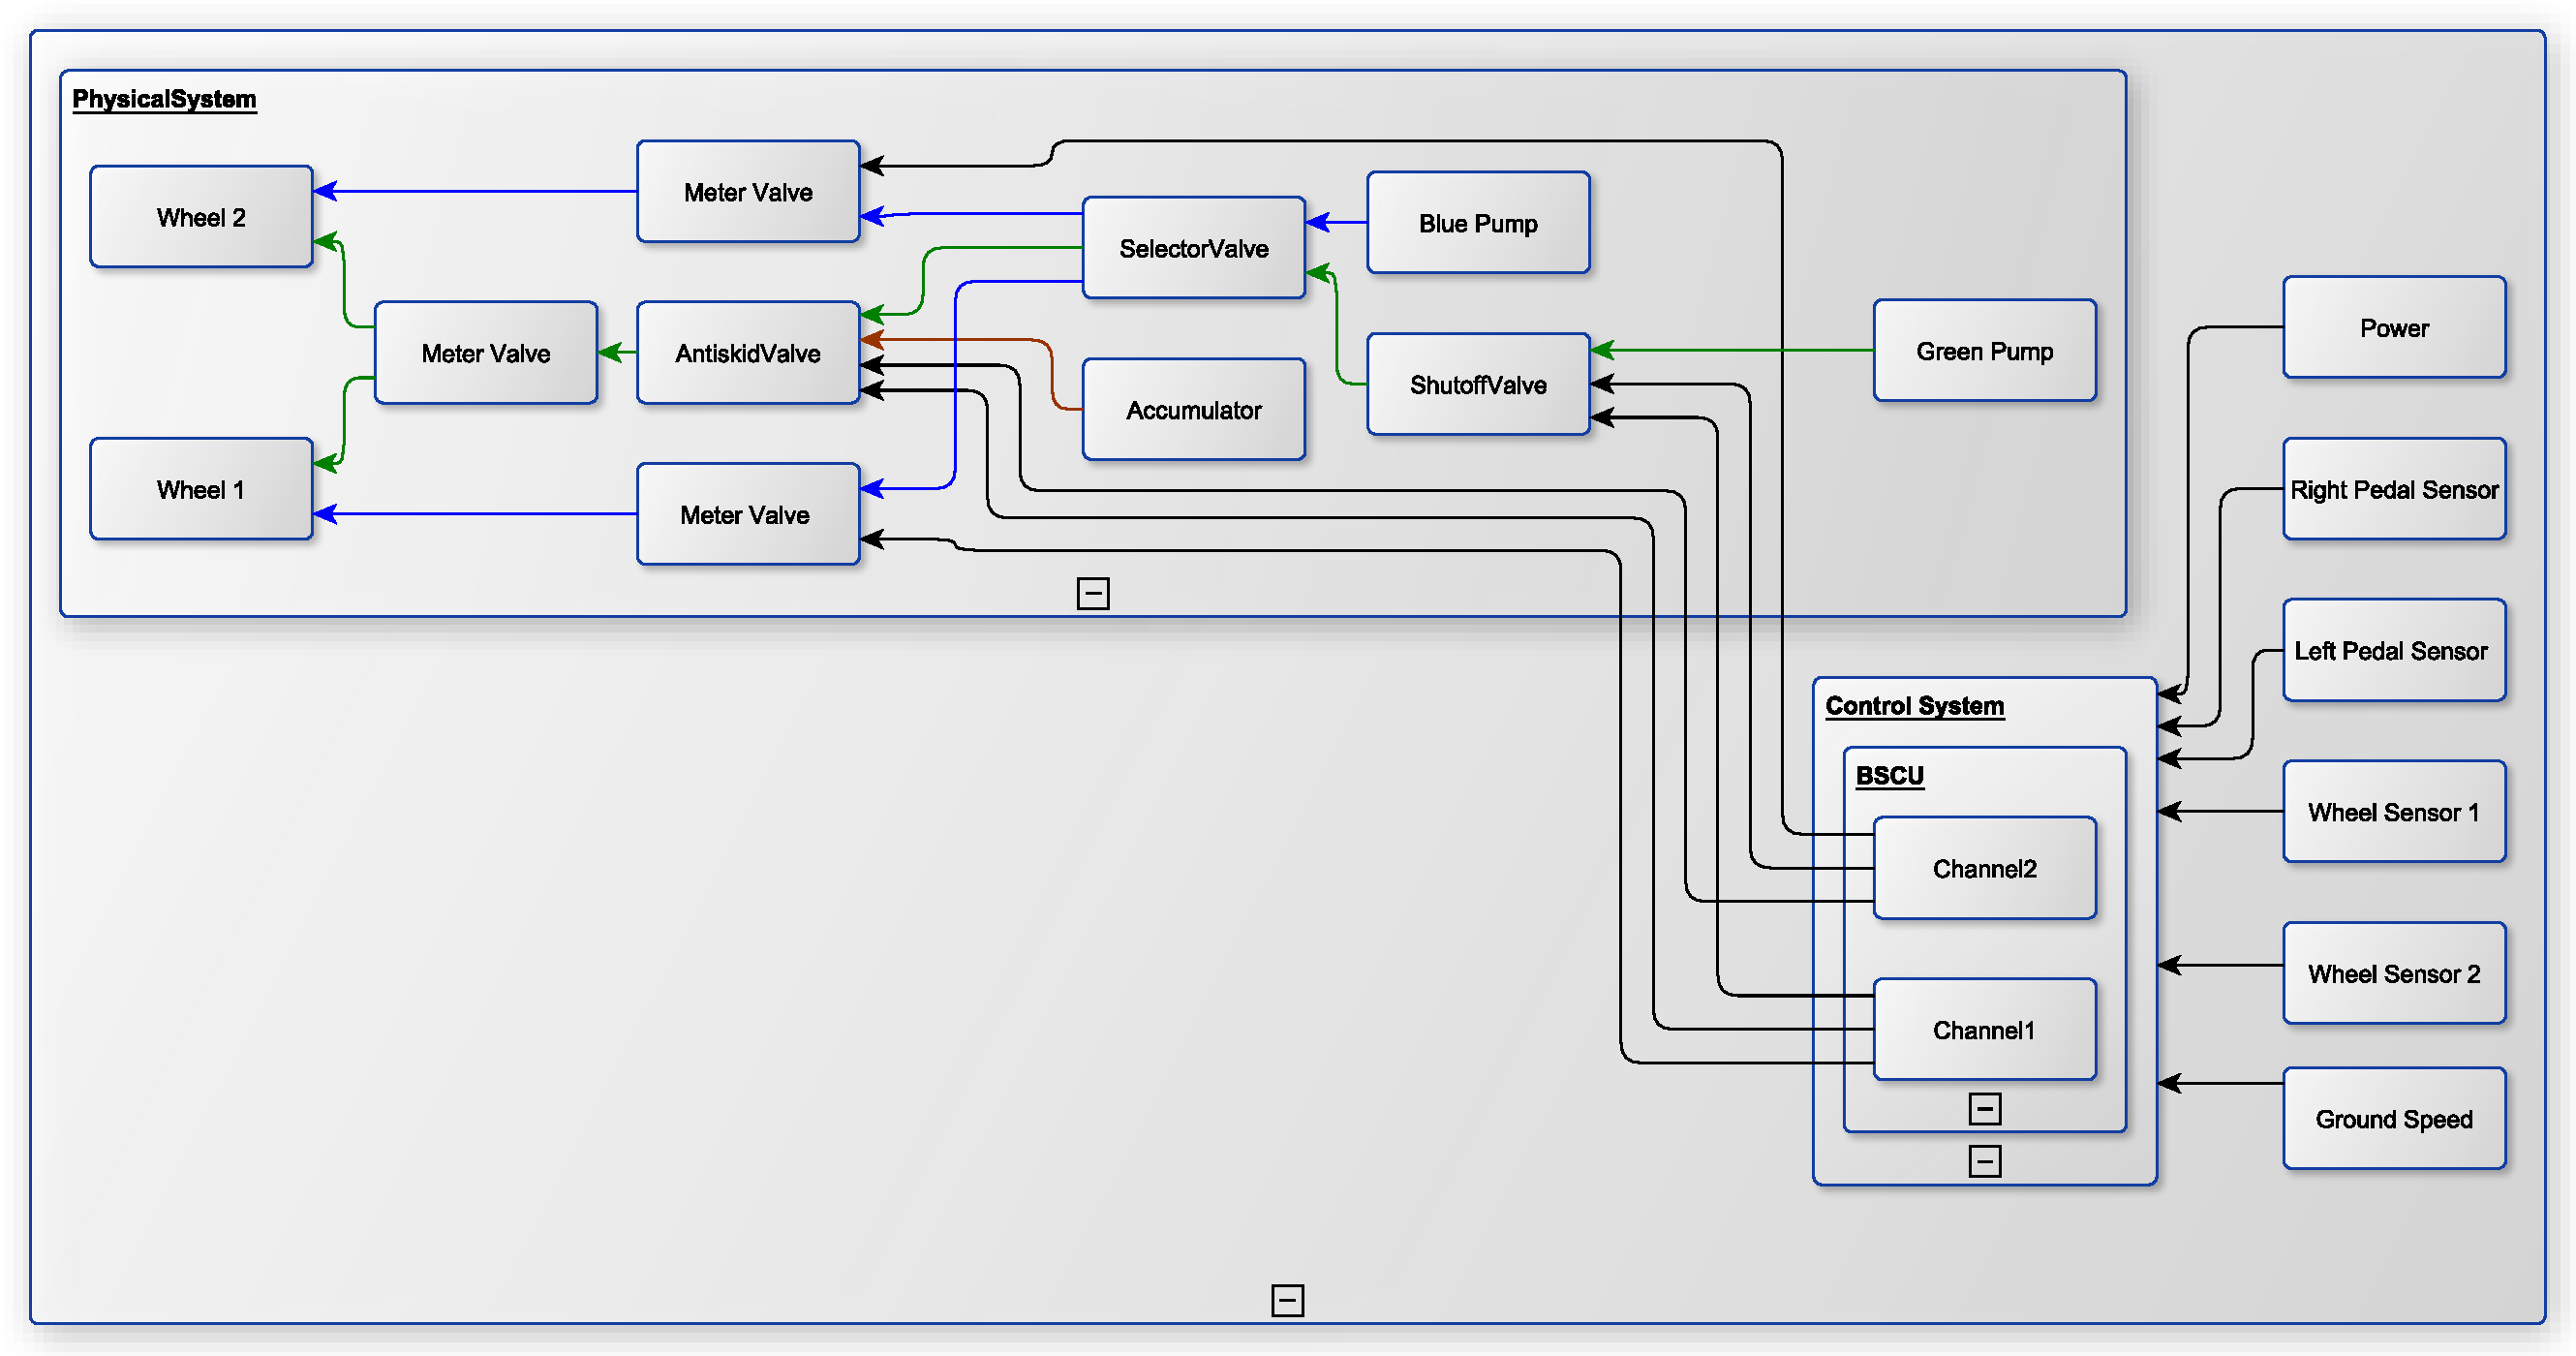
\includegraphics[trim=0 9 0 5,clip,width=\textwidth]{images/wbs_arch.pdf}
	\caption{Wheel Brake System}
	\label{fig:wbs}
\end{figure} 

%\subsubsection{WBS Architecture Description}
The WBS is composed of two main parts: the control system and the physical system. The control system electronically controls the physical system and contains a redundant channel of the Braking System Control Unit (BSCU) in case of failure. It also commands antiskid braking in case of skidding on the ground. The physical system consists of the hydraulic circuits running from hydraulic pumps to wheel brakes as well as valves that control the hydraulic fluid flow. This is what provides braking force to each of the 8 wheels of the aircraft. The wheels are all mechanically braked in pairs (one pair per landing gear). For simplicity's sake, Figure~\ref{fig:wbs} displays only two of the 8 wheels. 

There are three operating modes in the WBS model. In \textit{normal} mode, the system uses the \textit{green} hydraulic circuit. The normal system is composed of the green hydraulic pump and one meter valve per each of the 8 wheels. Each of the meter valves are controlled through electronic commands coming from the active channel of the BSCU. These signals provide braking and antiskid commands for each wheel. The braking command is determined through a sensor on the pilot pedal position and is labeled as \textit{Left/Right Pedal Sensor} in Figure~\ref{fig:wbs} and the antiskid command is determined by the \textit{Wheel Sensors}. 

In \textit{alternate} mode, the system uses the \textit{blue} hydraulic circuit. The alternate system is composed of the blue hydraulic pump, four meter valves, and four antiskid shutoff valves: one for each landing gear. The meter valves are mechanically commanded through the pilot pedal corresponding to each landing gear. If the system detects lack of pressure in the green circuit, the BSCU channel commands the selector valve to switch to the blue circuit. %This switch can occur, for example, if there is a lack of pressure from the green hydraulic pump, the green hydraulic pump circuit fails, or pressure is cut off by a shutoff valve. 
If the BSCU channel becomes invalid, the shutoff valve closes and we move into alternate mode. Once this system switches into alternate mode, it does not return to normal operation mode.

The last mode of operation of the WBS is the \textit{emergency} mode. This mode is entered if the blue hydraulic pump fails. The accumulator pump has a reserve of pressurized hydraulic fluid and will supply this to the blue circuit in emergency mode.

To get an idea of the size of this model, the system model contains 30 different kinds of components, 169 component instances, and a model depth of 5 hierarchical levels. 

The behavioral model is encoded using the AGREE annex and the behavior is based on descriptions found in AIR6110. The top level system properties are given by the requirements and safety objectives given in AIR6110. All of the subcomponent contracts support these system safety objectives through the use of assumptions on component input and guarantees on the output.

\begin{comment}
\subsubsection{WBS Behavioral Model Description}
\label{subsubsec:wbs_behavior}
The behavioral model is encoded using the AGREE annex and the behavior is based on descriptions found in AIR6110. The top level system properties are given by the requirements and safety objectives given in AIR6110. All of the subcomponent contracts support these system safety objectives by constraining subcomponent output behavior. 

Based on descriptions provided in AIR6110, the Functional Hazard Assessment (FHA) revealed a number of top level properties for the system. We will focus on one in the following sections in order to illustrate the use of the Safety Annex in fault modeling and how the behavioral propagation of faults can affect the top level safety properties of a system. 

One of the failure conditions described in AIR6110 is \textit{Inadvertent wheel braking of all wheels during takeoff roll after V1 shall be less than 1E-9 per takeoff}. Due to the catastrophic classification of this hazard, this is a property we chose for illustrative purposes. 

This property can be broken down as follows. In order for no inadvertent braking to occur, there needs to be a series of things that occur in the system simultaneously. The system is provided with both power and hydraulic pressure and the pilot has not commanded braking (by pressing the pedal). At the same time, the ground is moving (the plane is not stopped), there is braking force at the wheel, and the wheel is rolling. When all of these things happen together, this is inadvertant braking. Naturally, the safety property states this as all of these things do \textit{not} occur together. Given a model of this size, it can be complicated to determine the combinations of component errors that could occur in order to lead to a functional failure. 

In the following section, we outline the fault modelling process using the Safety Annex and illustrate using the WBS and some specific subcomponents.

%In the behavioral model, the lower level guarantees of the components serve to support the top level property. For example, in this property we have the following lower level component contracts that ensure that these behaviors of the system cannot occur simultaneously. \danielle{I need to run the lustre code using all IVCs to gather these supporting contracts. TODO: Get supporting contracts for this lemma, run analysis and see which of these supporting contracts are violated in the presence of which faults, explain the results.}


\end{comment}











\section{Fault Modeling with the Safety Annex}
\label{sec:fault_modeling}

To demonstrate the fault modeling capabilities of the Safety Annex we will use the Wheel Brake System (WBS) described in AIR6110~\cite{AIR6110}.  This system is a well-known example that has been used as a case study for safety analysis, formal verification, and contract based design~\cite{DBLP:conf/cav/BozzanoCPJKPRT15, 10.1007/978-3-319-11936-6-7, CAV2015:BoCiGrMa, Joshi05:SafeComp}. %The preliminary work for the safety annex was based on a simple model of the WBS~\cite{Stewart17:IMBSA}. To demonstrate a more complex fault modeling process, we constructed a functionally and structurally equivalent AADL version of one of the more complex WBS NuSMV/xSAP model (arch4wbs)~\cite{DBLP:conf/cav/BozzanoCPJKPRT15}.    

\begin{figure}[h!]
	\centering
	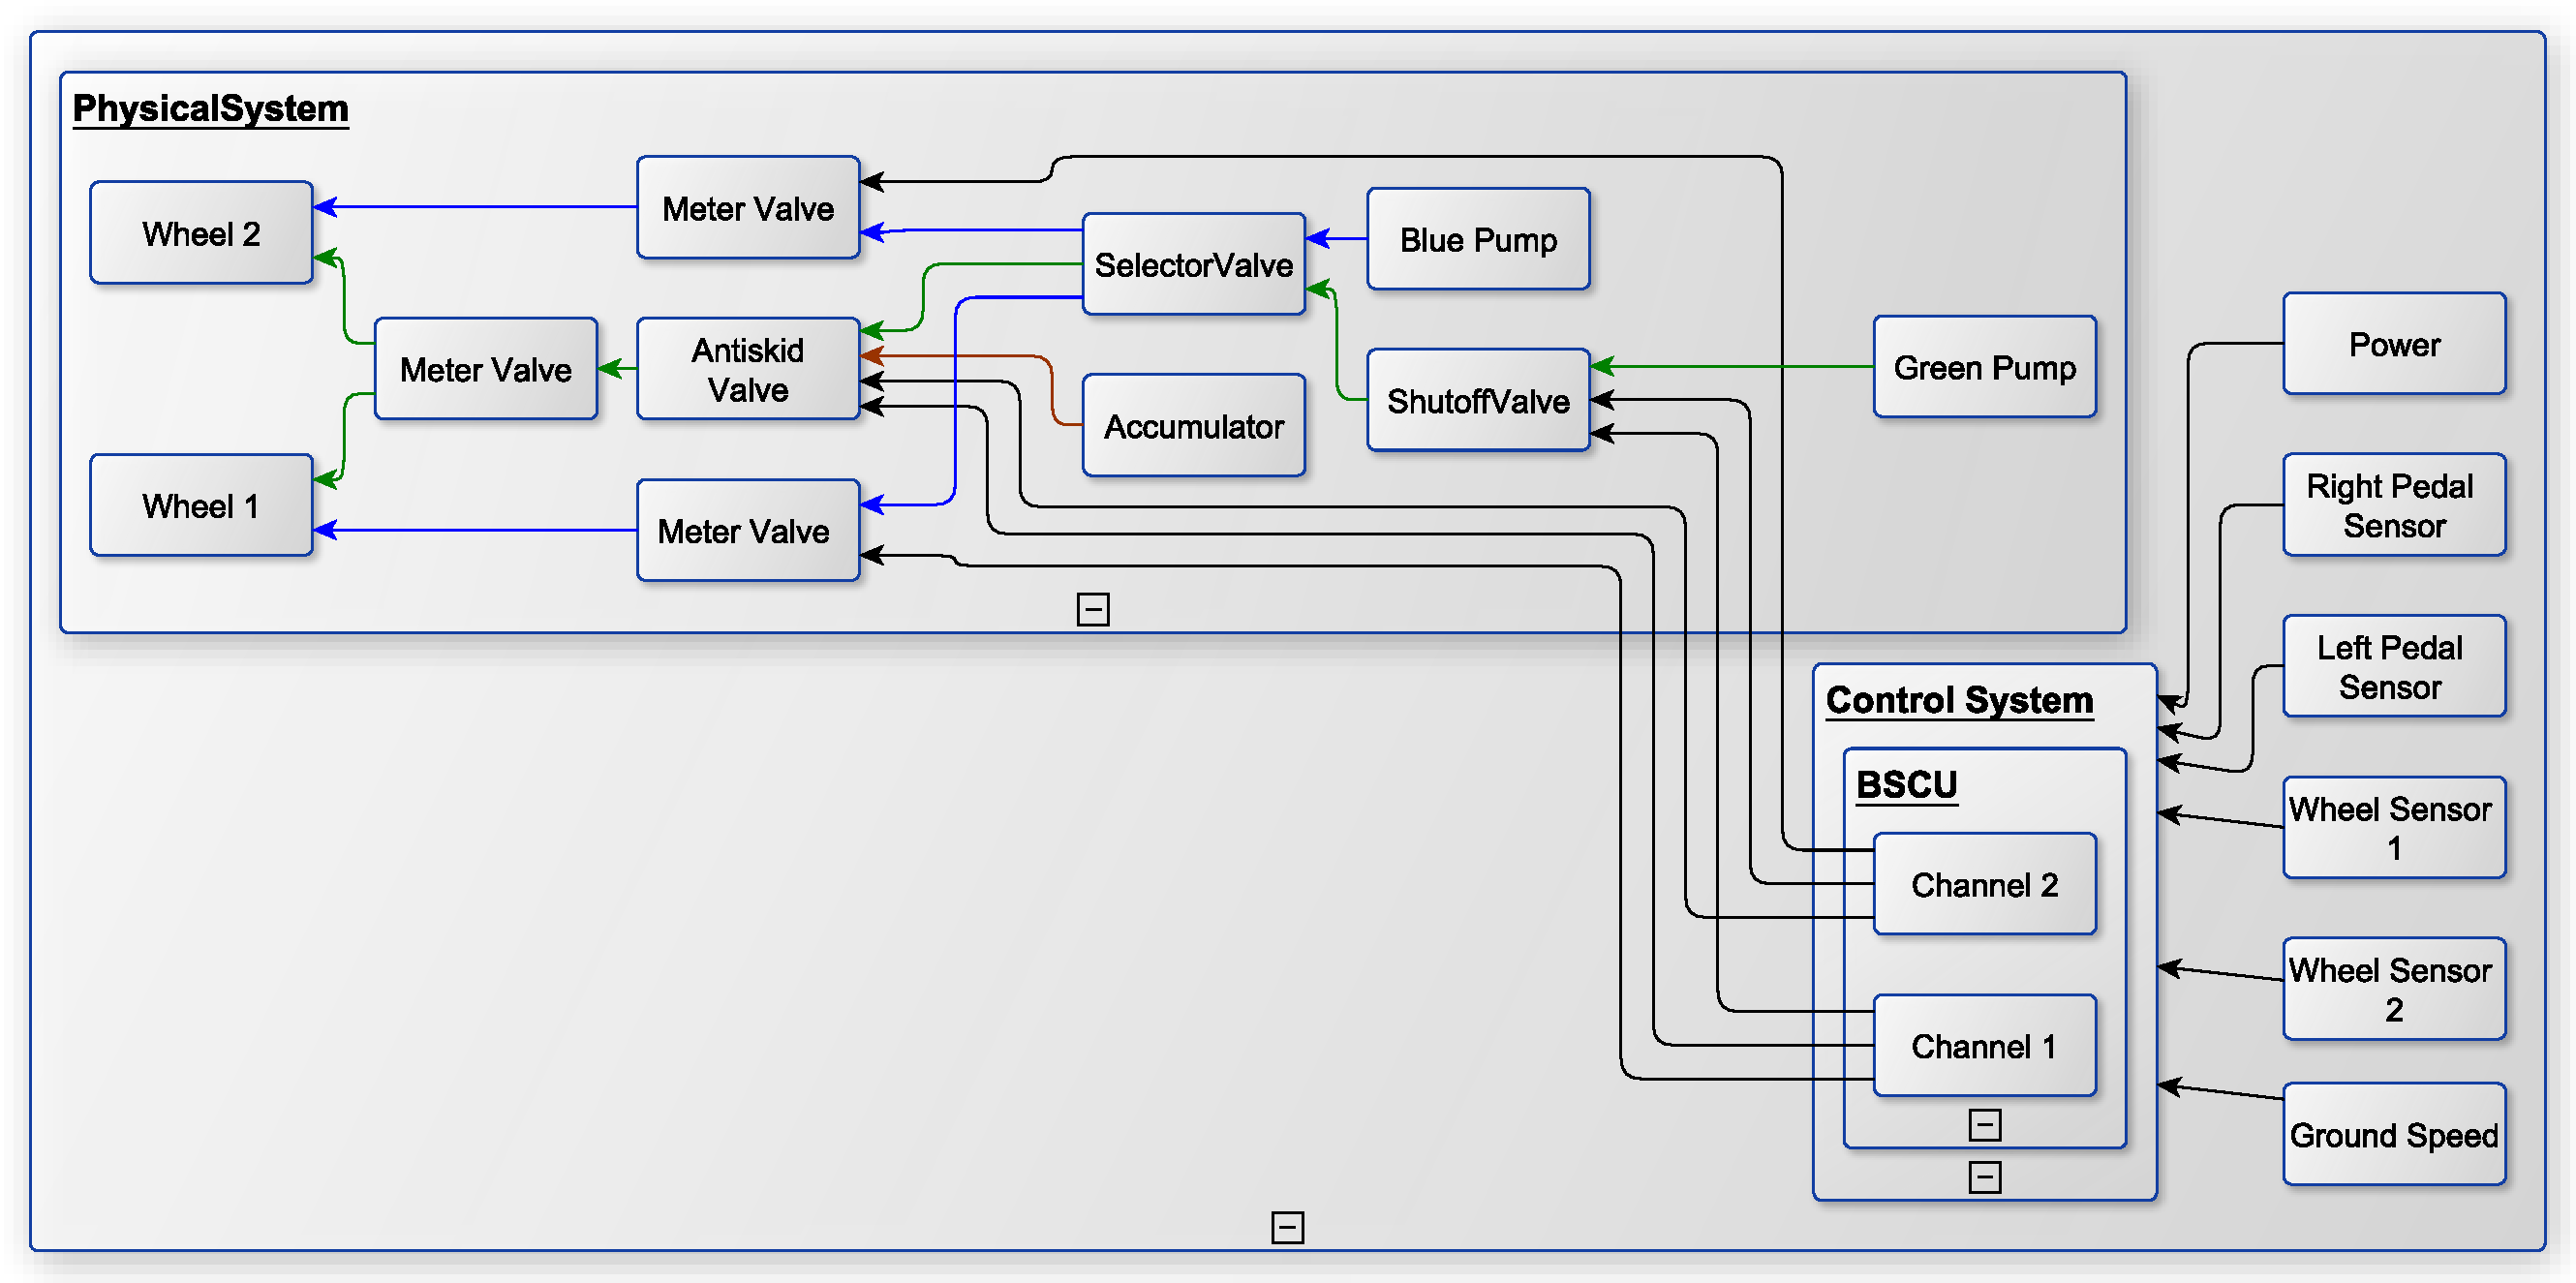
\includegraphics[trim=0 9 0 5,clip,width=\textwidth]{images/wbs_arch4_diagram.pdf}
	\caption{Wheel Brake System}
	\label{fig:wbs}
\end{figure} 

The WBS is composed of two main parts: the control system and the physical system. The control system electronically controls the physical system and contains a redundant channel of the Braking System Control Unit (BSCU) in case of failure. It also commands antiskid braking.% in case of skidding on the ground. 
The physical system consists of the hydraulic circuits running from hydraulic pumps to wheel brakes as well as valves that control the hydraulic fluid flow. This system provides braking force to each of the eight wheels of the aircraft. The wheels are all mechanically braked in pairs (one pair per landing gear). For simplicity, Figure~\ref{fig:wbs} displays only two of the eight wheels. 

There are three operating modes in the WBS model:

\begin{itemize}
	\renewcommand{\labelitemi}{\textbullet}
	\item In \textit{normal} mode, the system is composed of a \textit{green} hydraulic pump and one meter valve per each of the eight wheels. Each of the meter valves are controlled through electronic commands coming from the active channel of the BSCU. These signals provide braking and antiskid commands for each wheel. The braking command is determined through a sensor on the pedal and the antiskid command is determined by the \textit{Wheel Sensors}. 
	\item In \textit{alternate} mode, the system is composed of a \textit{blue} hydraulic pump, four meter valves, and four antiskid shutoff valves, one for each landing gear. The meter valves are mechanically commanded through the pilot pedal corresponding to each landing gear. If the system detects lack of pressure in the green circuit, the BSCU channel commands the selector valve to switch to the blue circuit. 
	\item In \textit{emergency} mode, the system mode is entered if the \textit{blue} hydraulic pump fails. The accumulator pump has a reserve of pressurized hydraulic fluid and will supply this to the blue circuit in emergency mode. 
\end{itemize}

The WBS architecture model in AADL contains 30 different kinds of components, 169 component instances, and a model depth of 5 hierarchical levels. 


%If the BSCU channel becomes invalid, the shutoff valve closes and we move into alternate mode. Once this system switches into alternate mode, it does not return to normal operation mode.

%There are three operating modes in the WBS model. In \textit{normal} mode, the system uses the \textit{green} hydraulic circuit. The normal system is composed of the green hydraulic pump and one meter valve per each of the eight wheels. Each of the meter valves are controlled through electronic commands coming from the active channel of the BSCU. These signals provide braking and antiskid commands for each wheel. The braking command is determined through a sensor on the pilot pedal position and is labeled as \textit{Left/Right Pedal Sensor} in Figure~\ref{fig:wbs} and the antiskid command is determined by the \textit{Wheel Sensors}. 

%In \textit{alternate} mode, the system uses the \textit{blue} hydraulic circuit. The alternate system is composed of the blue hydraulic pump, four meter valves, and four antiskid shutoff valves: one for each landing gear. The meter valves are mechanically commanded through the pilot pedal corresponding to each landing gear. If the system detects lack of pressure in the green circuit, the BSCU channel commands the selector valve to switch to the blue circuit. 
%If the BSCU channel becomes invalid, the shutoff valve closes and we move into alternate mode. Once this system switches into alternate mode, it does not return to normal operation mode.

%The last mode of operation of the WBS is the \textit{emergency} mode. This mode is entered if the blue hydraulic pump fails. The accumulator pump has a reserve of pressurized hydraulic fluid and will supply this to the blue circuit in emergency mode.

%The model contains 30 different kinds of components, 169 component instances, a model depth of 5 hierarchical levels.  The model includes one top-level assumption and  11 top-level system properties, with 113 guarantees allocated to subsystems.  There are a total of 33 different fault types and 141 fault instances within the model.  The large number of fault instances is due to the redundancy in the system design and its replication to control 8 wheels.

The behavioral model is encoded using the AGREE annex and the behavior is based on descriptions found in AIR6110. The top level system properties are given by the requirements and safety objectives in AIR6110. All of the subcomponent contracts support these system safety objectives through the use of assumptions on component input and guarantees on the output. The WBS behavioral model in AGREE annex includes one top-level assumption and  11 top-level system properties, with 113 guarantees allocated to subsystems.  

An example system safety property is to ensure that there is no inadvertent braking of any of the wheels. This is based on a failure condition described in AIR6110 is \textit{Inadvertent wheel braking on one wheel during takeoff shall be less than 1E-9 per takeoff}. 
Inadvertent braking means that braking force is applied at the wheel but the pilot has not pressed the brake pedal.  In addition, the inadvertent braking requires that power and hydraulic pressure are both present, the plane is not stopped, and the wheel is rolling (not skidding). 
%in Figure~\ref{fig:inadvertent_braking}. 
The property is stated in AGREE such that inadvertent braking does \textit{not} occur, as shown below. 

\begin{figure}[h!]
	\vspace{-0.2in}
	\begin{center}
		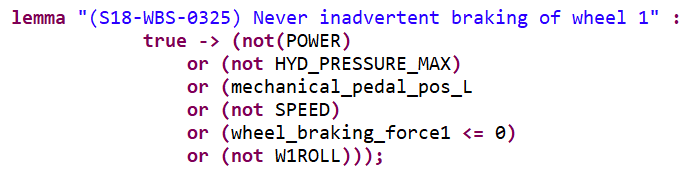
\includegraphics[width=.8\textwidth]{images/inadvertent_braking.png}
	\end{center}
	\vspace{-0.3in}
	%\caption{AGREE Contract for Top Level Property}
	\label{fig:inadvertent_braking}
	\vspace{-0.2in}
\end{figure}


\subsection{Component Fault Modeling}

The usage of the terms error, failure, and fault are defined in ARP4754A and are described here for ease of understanding~\cite{SAE:ARP4754A}. An \textit{error} is a mistake made in implementation, design, or requirements. A \textit{fault} is the manifestation of an error and a \textit{failure} is an event that occurs when the delivered service of a system deviates from correct behavior. If a fault is activated under the right circumstances, that fault can lead to a failure. The terminology used in EMV2 differs slightly for an error: an error is a corrupted state caused by a fault. The error propagates through a system and can  manifest as a failure. In this paper, we use the ARP4754A terminology with the added definition of \textit{error propagation} as used in EMV2. An error is a mistake made in design or code and an error propagation is the corrupted state caused by an active fault. 

The Safety Annex is used to add potential faulty behaviors to a component model.  When the fault is activated by its specified triggering conditions, it modifies the output of the component. This faulty behavior may violate the contracts of other components in the system, including assumptions of downstream components. The impact of a fault is computed by the AGREE model checker when the safety analysis is run on the fault model. Examples of such faults include valves being stuck open or closed, output of a software component being nondeterministic, or power being cut off. 
%Faulty components can be mechanical or digital, but in this section we focus on a digital component in the WBS -- a brake pedal position sensor component. 

One of the components important to the inadvertent braking property is the brake pedal. When the mechanical pedal is pressed, a sensor reads this information and passes an electronic signal to the BSCU which then commands hydraulic pressure to the wheels. 

%Figure~\ref{fig:sensor} 
Below shows the AADL pedal sensor component with a contract for its nominal behavior. The sensor has only one input, the mechanical pedal position, and one output, the electrical pedal position. %The 
A property that governs the behavior of the component is that the mechanical position should always equal the electronic position. 

\begin{figure}[h!]
	\hspace*{-2cm}
	\vspace{-0.55in} 
	\begin{center}
		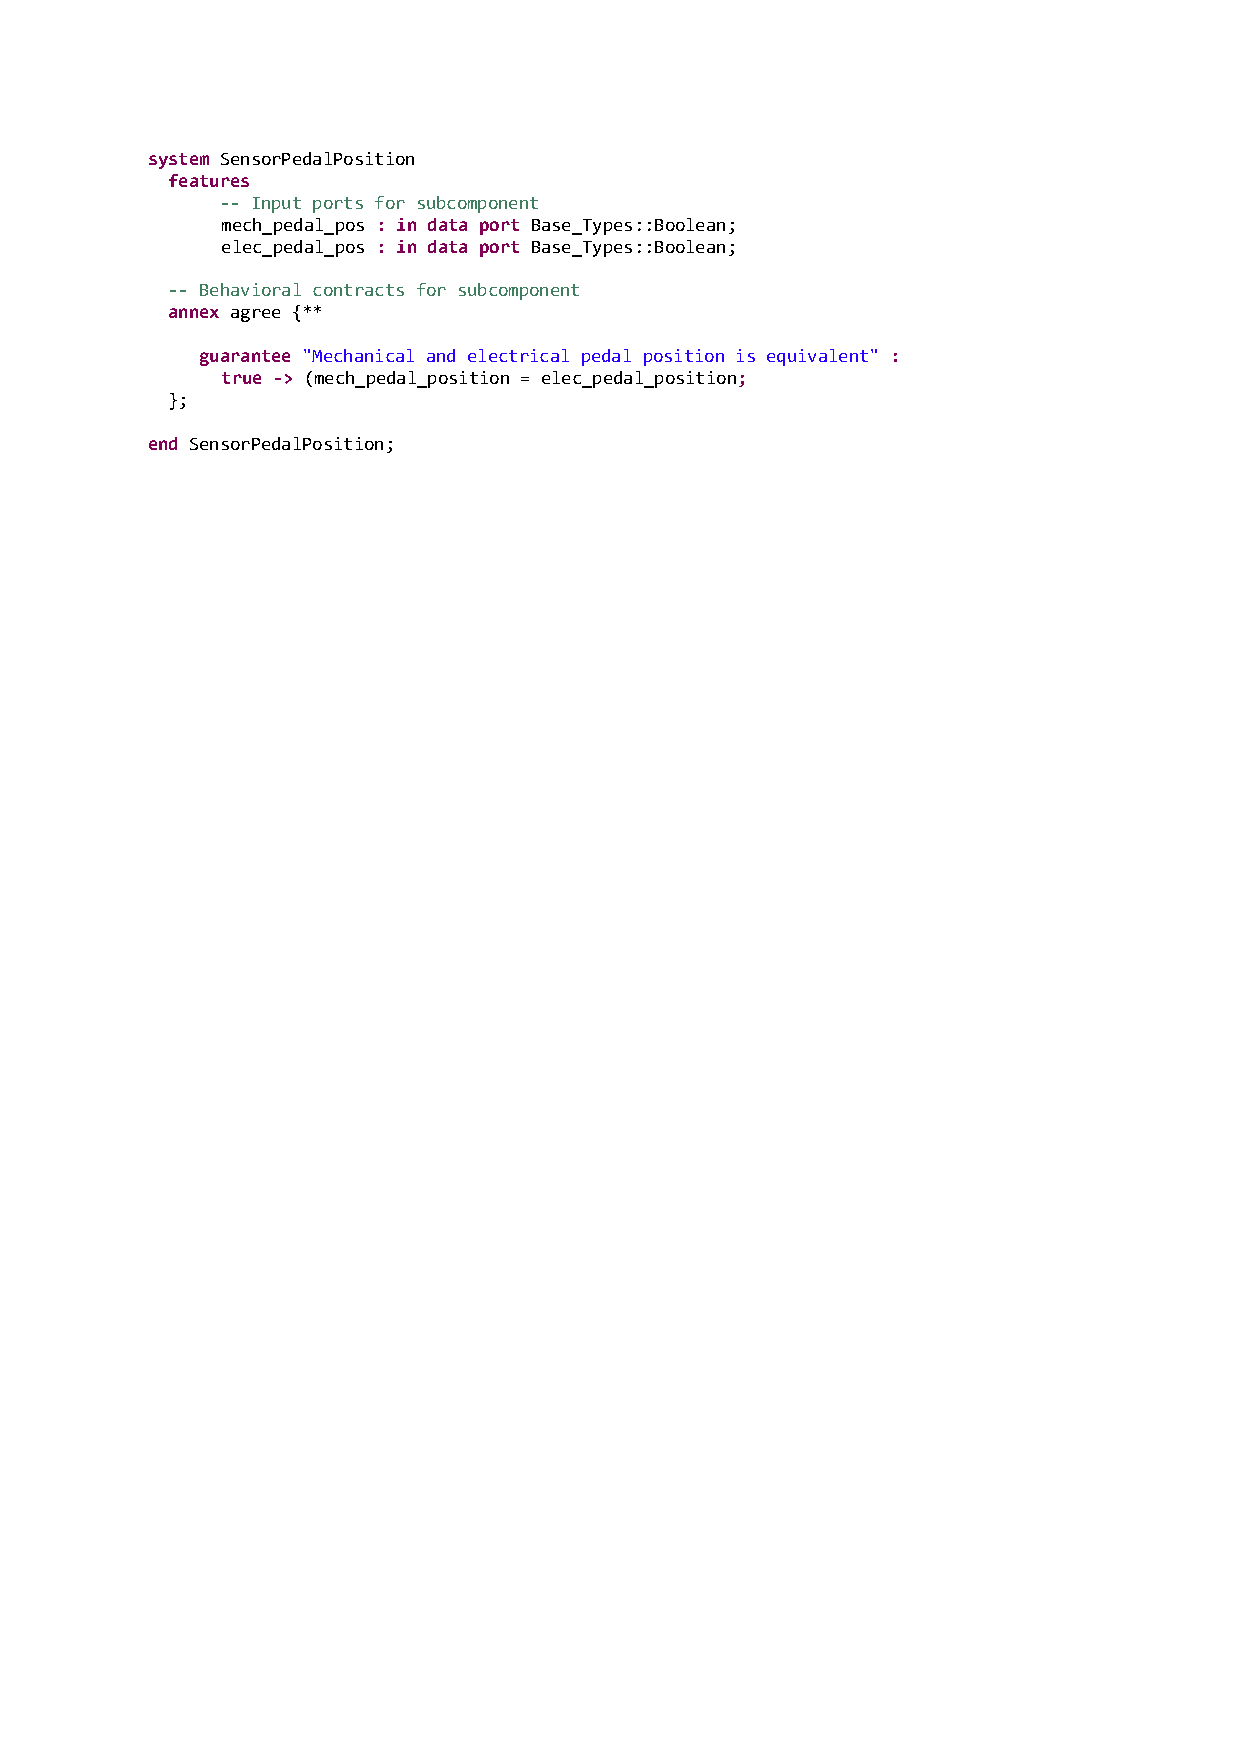
\includegraphics[trim=0 640 -10 70,clip,width=1.5\dimexpr\textwidth-2cm\relax]{images/system_sensor.pdf}
		\vspace{-0.3in}
	%	\caption{An AADL System Type: The Pedal Sensor}
		\label{fig:sensor}
	\end{center}
	\vspace{-0.4in}
\end{figure}

One possible failure for this sensor is inversion of its output value. This fault can be triggered with probability $5.0\times 10^{-6}$ as described in AIR6110 (in reality, the component failure probability is 
collected from hardware specification sheets).  %Figure~\ref{fig:sensorFault} 
The Safety Annex definition for this fault is shown below. Fault behaviors may be defined by the user or by using a library of fault nodes, in this case, \textit{inverted\_fail}.  When the fault is triggered, the nominal output of the component (\textit{elec\_pedal\_position}) is replaced with its failure value (\textit{val\_out}). 

\begin{figure}[h!]
	\hspace*{-2cm}
	\vspace{-0.5in} 
	\begin{center}
		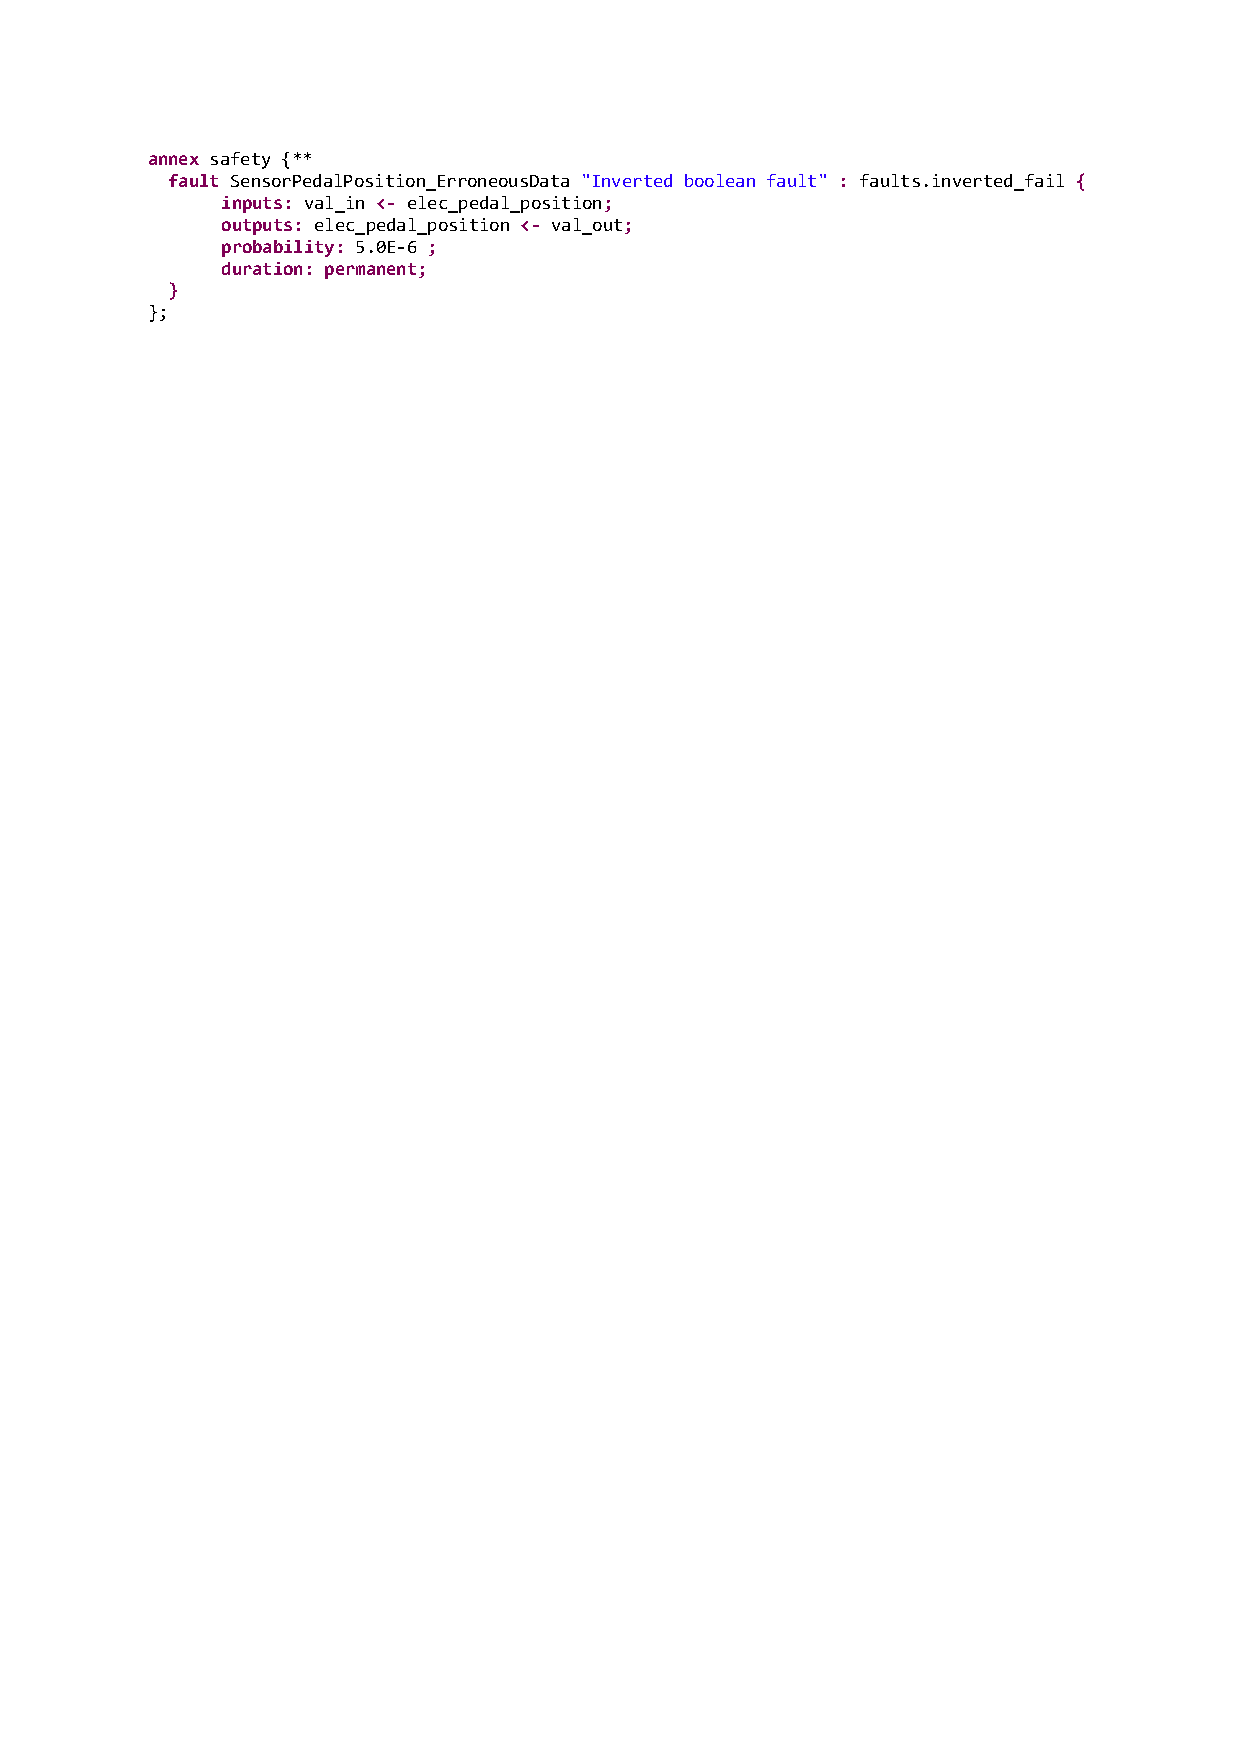
\includegraphics[trim=0 690 -10 70,clip,width=1.5\dimexpr\textwidth-2cm\relax]{images/safetyannex_sensorfault.pdf}
		\vspace{-0.3in}
		%\caption{The Safety Annex for the Pedal Sensor}
		\label{fig:sensorFault}
	\end{center}
	\vspace{-0.3in}
\end{figure}

The WBS fault model in Safety Annex contains a total of 33 different fault types and 141 fault instances. The large number of fault instances is due to the redundancy in the system design and its replication to control 8 wheels.

\subsection{Implicit %Failure
	Error Propagation}
In the Safety Annex approach, faults are captured as faulty behaviors that augment the system behavioral model in AGREE contracts. No explicit %fault
error propagation is necessary since the faulty behavior itself propagates through the system just as in the nominal system model. The effects of any triggered fault are manifested through analysis of the AGREE contracts. 

On the contrary, in the AADL Error Model Annex, Version 2 (EMV2)~\cite{EMV2} approach, all errors must be explicitly propagated through each component (by applying fault types on each of the output ports) in order for a component to have an impact on the rest of the system. To illustrate the key differences between implicit %failure
error propagation provided in Safety Annex and the explicit %failure 
error propagation provided in EMV2, we use a simplified behavioral flow from the WBS example using code fragments from EMV2, AGREE, and the Safety Annex. 

\begin{figure}[t]
	\vspace{-0.19in}
	\centering
	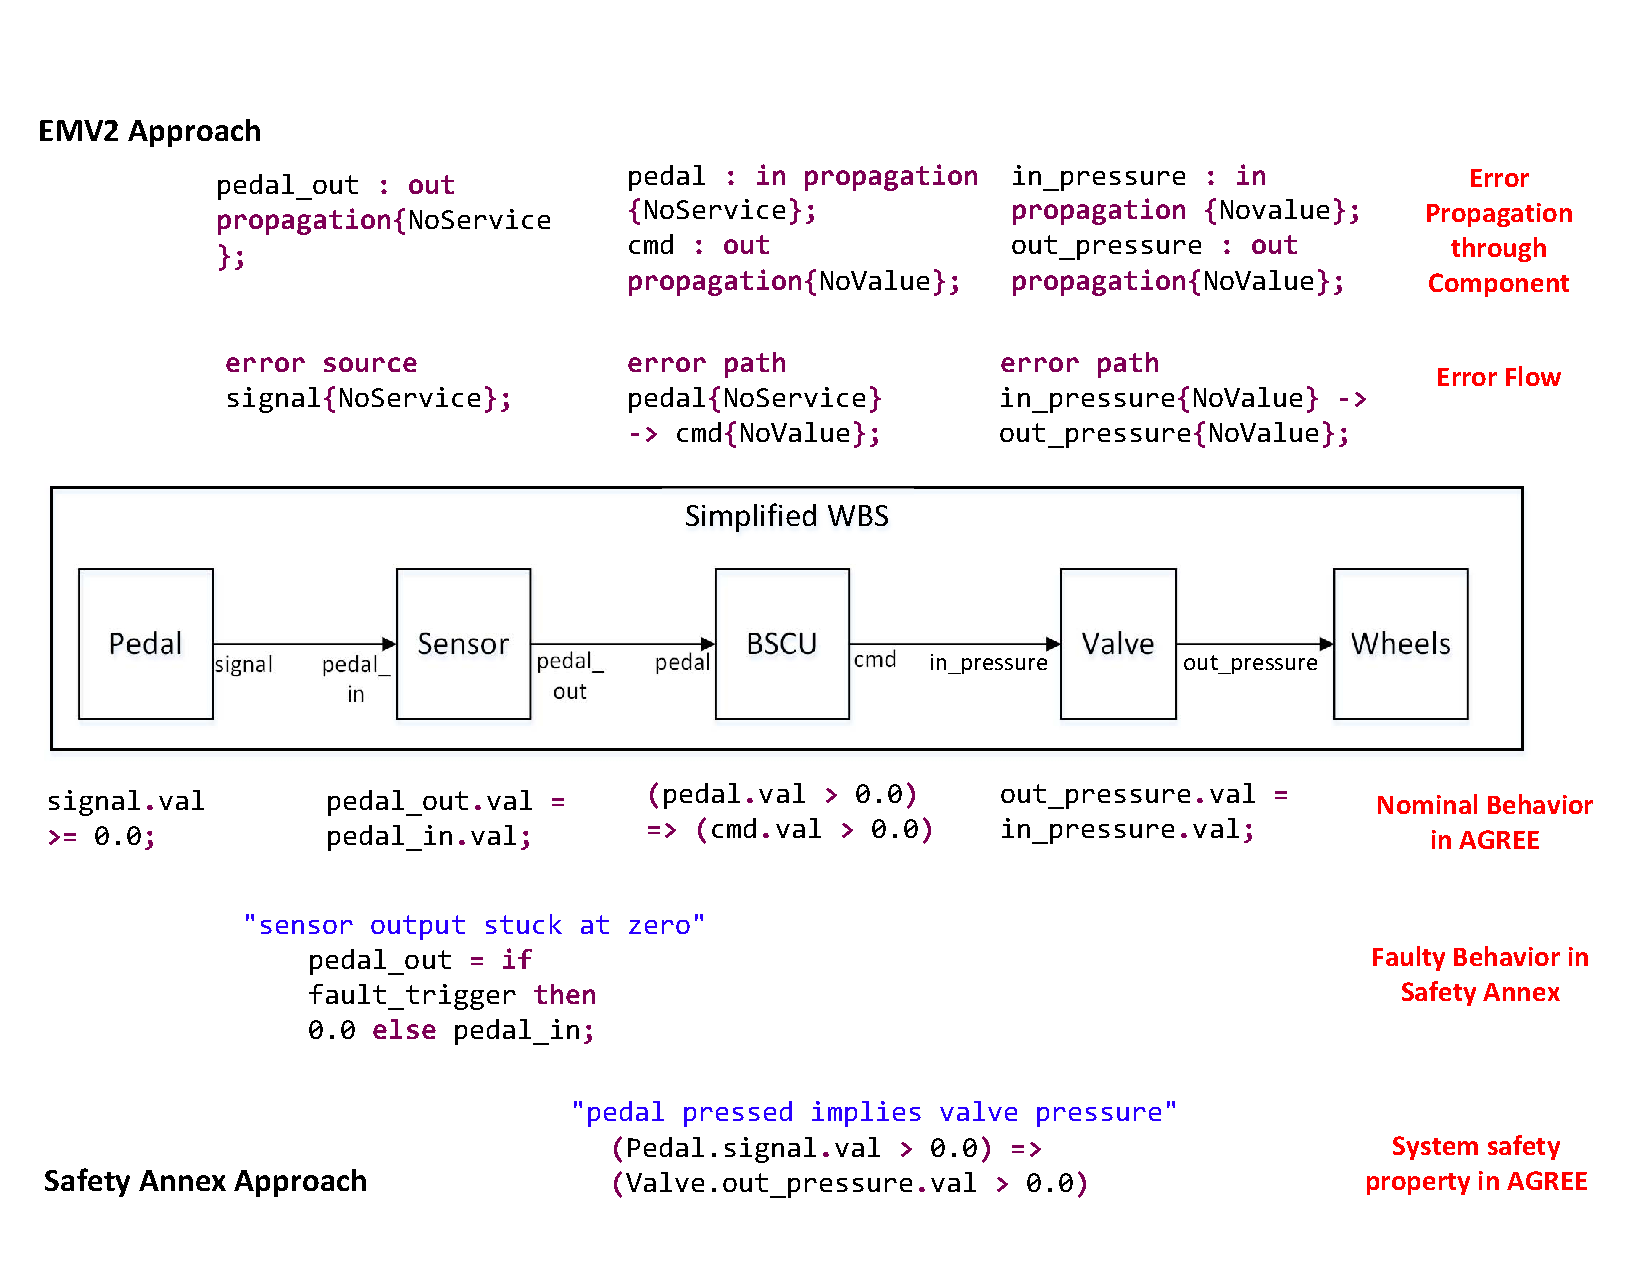
\includegraphics[trim=0 9 0 5,clip,width=\textwidth]{images/Comparison_with_EMV2.pdf}
	\vspace{-0.3in}
	\caption{Differences between Safety Annex and EMV2}
	\label{fig:comparison_with_EMV2}
	\vspace{-0.2in}
\end{figure} 

In this simplified WBS system, the physical signal from the Pedal component is detected by the Sensor and the pedal position value is passed to the Braking System Control Unit (BSCU) components.  The BSCU generates a pressure command to the Valve component which applies hydraulic brake pressure to the Wheels. 

In the EMV2 approach (top half of Figure~\ref{fig:comparison_with_EMV2}), the ``NoService'' fault is explicitly propagated through all of the components. These fault types are essentially tokens that do not capture any analyzable behavior. At the system level, analysis tools supporting the EMV2 annex can aggregate the propagation information from different components to compose an overall fault flow diagram or fault tree. 

When a fault is triggered in the Safety Annex (bottom half of Figure~\ref{fig:comparison_with_EMV2}), the output behavior of the Sensor component is modified. In this case the result is a ``stuck at zero'' error. The behavior of the BSCU receives a zero input and proceeds as if the pedal has not been pressed. This will cause the top level system contract to fail: {\em pedal pressed implies brake pressure output is positive}.

\begin{comment}
%\subsection{Comparison to the AADL Error Annex}

The AADL language has previously been extended to provide some fault modeling and analysis capabilities using its Error Model Annex, Version 2 (EMV2)~\cite{EMV2}.  EMV2 focuses on injection and propagation of discrete faults for generation of fault trees, rather than on analysis of system behavior in the presence of faults. 
To illustrate some of the key differences between our approach and the EMV2 approach, Figure~\ref{fig:comparison_with_EMV2} shows a simplified  behavioral flow with code fragments from EMV2, AGREE, and the Safety Annex. 

\begin{figure}[t]
	\vspace{-0.45in}
	\centering
	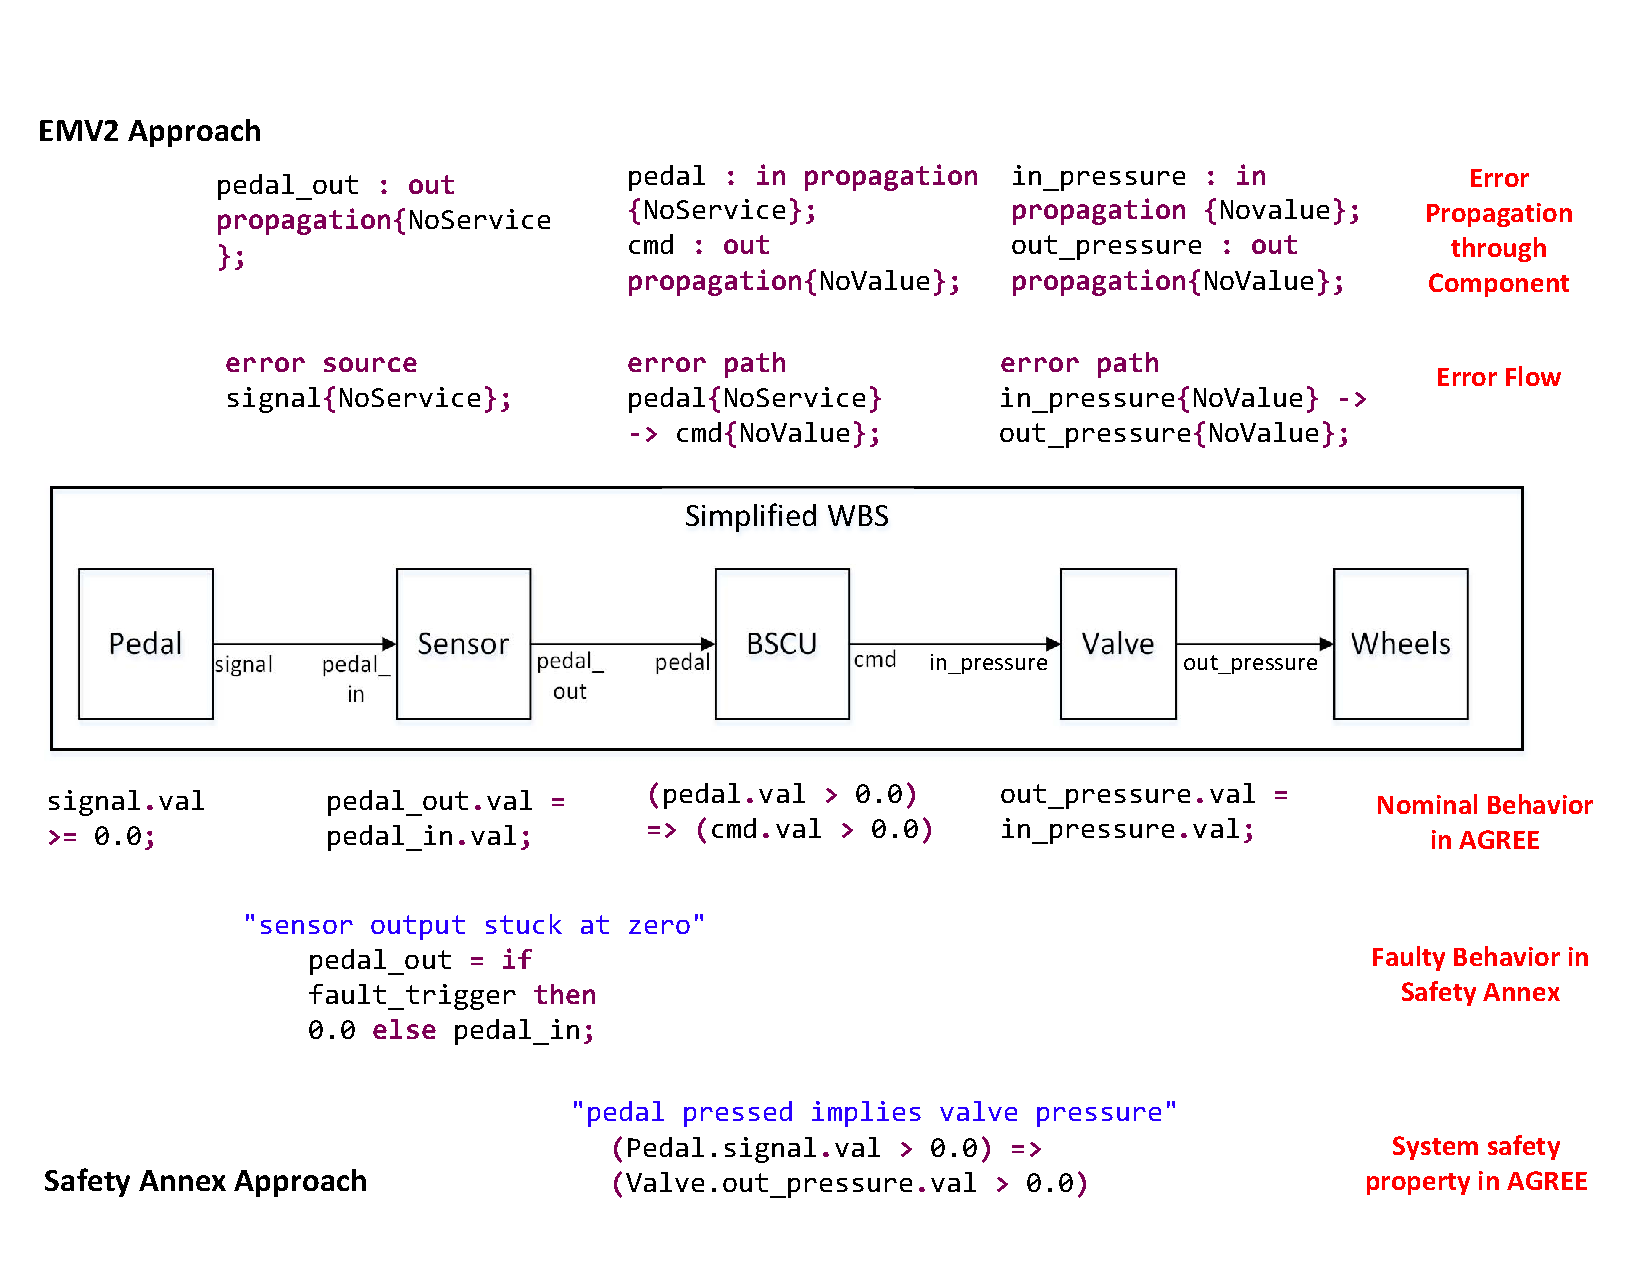
\includegraphics[trim=0 9 0 5,clip,width=\textwidth]{images/Comparison_with_EMV2.pdf}
	%\vspace{0.4in}
	\caption{Differences between Safety Annex and EMV2}
	\label{fig:comparison_with_EMV2}
\end{figure} 

In this simplified WBS system, the physical signal from the Pedal component is detected by the Sensor, and the pedal position value is passed to the Braking System Control Unit (BSCU) components.  The BSCU generates a pressure command to the Valve component which applies hydraulic brake pressure to the Wheels. 

In the EMV2 approach (top half of Figure~\ref{fig:comparison_with_EMV2}), all errors must be explicitly propagated through each component (by applying fault types on each of the output ports) in order for a component to have an impact on the rest of the system. In the example, the ``NoService'' fault is explicitly allowed by the EMV2 declarations to propagate through all of the components.  These fault types are essentially tokens that do not capture any analyzable behavior.  At the system level, analysis tools supporting the EMV2 annex can aggregate the fault flow and propagation information from different components to compose an overall fault flow diagram or fault tree.

In the Safety Annex approach (bottom half of Figure~\ref{fig:comparison_with_EMV2}), faults augment the system behavioral model through the AGREE contracts.  When a fault is triggered, the output behavior of the Sensor component is modified, in this case resulting a ``stuck at zero'' error. The behavior of the BSCU receives a zero input and proceeds as if the pedal has not been pressed. This will cause the top level system contract to fail: {\em pedal pressed implies brake pressure output is positive}. No explicit propagation is necessary since the faulty behavior propagates through the system just as in the nominal system model. The system and component failures are manifested through analysis of the AGREE contracts. 
\end{comment}

\subsection{Explicit %Failure 
	Error Propagation} 
%Faults
Failures in hardware (HW) components can trigger behavioral faults in the system components that depend on them. For example, a CPU %fault
Failure may trigger faulty behavior in the threads bound to that CPU. In addition, a %fault
failure in one HW component may trigger %faults
failure in other HW components located nearby, such as overheating, fire, or explosion
in the containment location. 
The Safety Annex provides the capability to explicitly model the impact of hardware %faults
failures on other faults, behavioral or non behavioral. The explicit propagation to non behavioral faults is similar to that provided in EMV2.

To better model %HW dependent faults 
faults at the system level dependent on HW failures, a fault model element is introduced called a \textit{hardware fault}. Users are not required to specify behavioral effects for the HW faults, nor are data ports necessary on which to apply the fault definition. An example of a model component fault declaration is shown below:
\begin{figure}[h!]
	\vspace{-0.2in}
	\begin{center}
	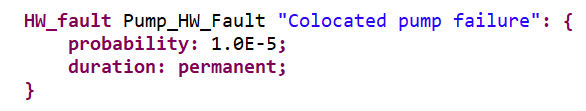
\includegraphics[width=.7\textwidth]{images/hw_fault2.png}
	\end{center}
	\vspace{-0.3in}
	%\caption{Hardware Fault Definition}
	\label{fig:hwFault}
	%\vspace{-0.2in}
	\vspace{-0.1in}
\end{figure}

Users specify dependencies between the HW component faults and faults that are defined in other components, either HW or SW. The hardware fault then acts as a trigger for dependent faults. This allows a simple propagation from the faulty HW component to the SW components that rely on it, affecting the behavior on the outputs of the affected SW components.

%As an example, we will look yet again at the WBS. 
In the WBS example, assume that both the green and blue hydraulic pumps are located in the same compartment in the aircraft and an explosion in this compartment rendered both pumps inoperable.
%An accident took place and the green (normal) hydraulic pump took the force of an explosion. When the green hydraulic pump exploded, the pump shrapnel flew into the blue pump and it became from then on unoperable. 
The HW fault definition can be modeled first in the green hydraulic pump component as shown in Figure~\ref{fig:hwFault}. The activation of this fault triggers the activation of related faults as seen in the \textit{propagate\_to} statement shown below. % in Figure~\ref{fig:hwFaultProp}. 
Notice that these pumps need not be connected through a data port in order to specify this propagation. %Furthermore, the probability of the HW fault activation can be specified. 

\begin{figure}[h!]
	\vspace{-0.2in}
	\begin{center}
		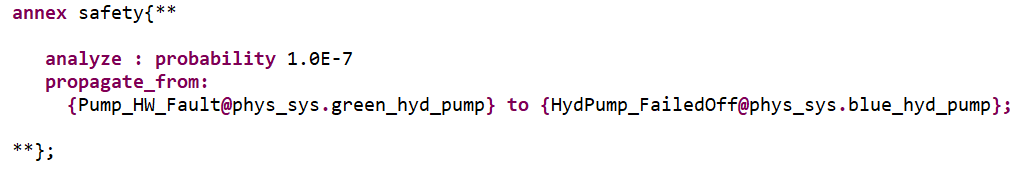
\includegraphics[width=1.0\textwidth]{images/hw_prop_stmt.png}
	\end{center}
	\vspace{-0.3in}
	%\caption{Hardware Fault Propagation Statement}
	\label{fig:hwFaultProp}
	%\vspace{-0.2in}
	\vspace{-0.1in}
\end{figure}

The fault dependencies are specified in the system implementation where the system configuration that causes the dependencies becomes clear (e.g., binding between SW and HW components, co-location of HW components). 
%This is because fault propagations are typically tied to the way components are connected or bound together; this information may not be available when faults are being specified for individual components. Having fault propagations specified outside of a component’s fault statements also makes it easier to reuse the component in different systems. 


\begin{comment}
\subsection{Fault Hypothesis}

An annotation in the AADL model determines the fault hypothesis. This may specify either a maximum number of faults that can be active at any point in execution (see Figure~\ref{fig:hwFaultProp}) or that only faults whose probability of simultaneous occurrence is above some probability threshold should be considered. Tying back to traditional safety analysis, the former is analogous to restricting the cutsets to a specified maximum number of terms, and the latter is analogous to restricting the cutsets to only those whose probability is above some set value.

In the former case, we assert that the sum of the true {\em fault\_\_trigger} variables is below some integer threshold.  In the latter, we determine all combinations of faults whose probabilities are above the specified probability threshold, and describe this as a proposition over {\em fault\_\_trigger} variables. 
%
With the introduction of dependent faults, active faults are divided into two categories: independently active (activated by its own triggering event) and dependently active (activated when the faults they depend on become active). The top level fault hypothesis applies to independently active faults. Faulty behaviors augment nominal behaviors whenever their corresponding faults are active (either independently active or dependently active).
\end{comment}










\section{Architecture and Implementation}
\label{sec:implementation}

The architecture of the Safety Annex is shown in Figure~\ref{fig:plugin-arch}.  It is written in Java as a plug-in for the OSATE AADL toolset, which is built on Eclipse.  It is not designed as a stand-alone extension of the language, but works with behavioral contracts specified in AGREE AADL annex and associated tools~\cite{NFM2012:CoGaMiWhLaLu}.  AGREE allows {\em assume-guarantee} behavioral contracts to be added to AADL components.  The language used for contract specification is based on the Lustre dataflow language~\cite{Halbwachs91:IEEE}. AGREE improves scalability of formal verification to large systems by decomposing the analysis of a complex system architecture into a collection of smaller verification tasks that correspond to the structure of the architecture.

\begin{figure}
	\begin{center}
		%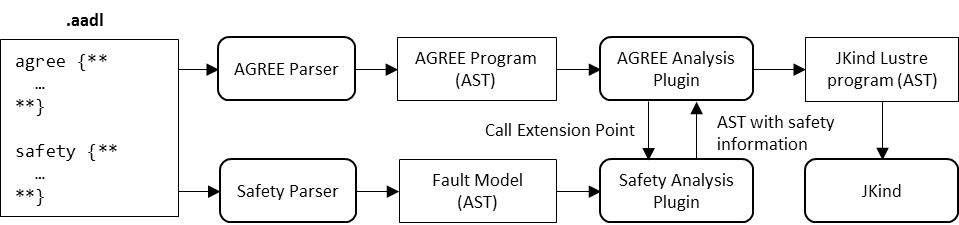
\includegraphics[trim=0 400 430 0,clip,width=0.85\textwidth]{images/arch.png}
		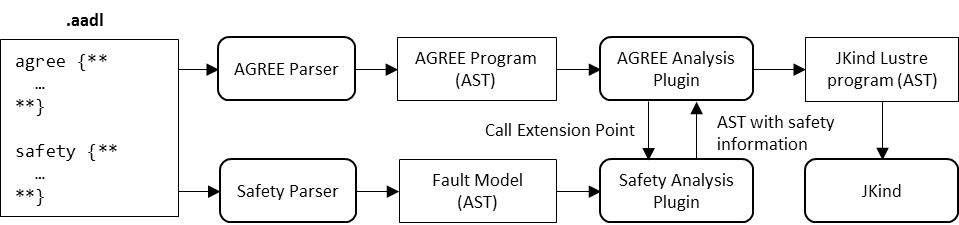
\includegraphics[width=.9\textwidth]{images/arch.png}
	\end{center}
	\vspace{-0.2in}
	\caption{Safety Annex Plug-in Architecture}
	\label{fig:plugin-arch}
\end{figure}

AGREE contracts are used to define the nominal behaviors of system components as {\em guarantees} that hold when {\em assumptions} about the values the component's environment are met.  The Safety Annex extends these contracts to allow faults to modify the behavior of component inputs and outputs.  To support these extensions, AGREE implements an Eclipse extension point interface that allows other plug-ins to modify the generated abstract syntax tree (AST) prior to its submission to the solver.  If the Safety Annex is enabled, these faults are added to the AGREE contract and, when triggered, override the nominal guarantees provided by the component.  

An example of a portion of an initial AGREE node and its extended contract is shown in Figure~\ref{fig:lustre}.  %The \texttt{\_\_fault} variables and declarations are added to allow the contract to override the nominal behavioral constraints (provided by guarantees) on outputs.  In the Lustre language, \texttt{assertion}s are constraints that are assumed to hold in the transition system. 
In the left column of the figure, the nominal Lustre pump definition is shown with an AGREE contract on the output. In the right column, the additional local variables for the fault are seen in boxes 1 and 2, the assertion binding the fault value to the nominal value is seen in boxes 3 and 4, and the fault node definition is given in box 5. 

%A  benefit of utilizing the AGREE behavioral annex is the ability to perform both monolithic and compositional analysis on the nominal model. AGREE allows {\em assume-guarantee} behavioral contracts to be added to AADL components.  The language used for contract specification is based on the Lustre dataflow language~\cite{Halbwachs91:IEEE} and the nominal model (AADL model annotated with AGREE contracts) is translated into Lustre before being sent to the JKind model checker for verification\cite{2017arXiv171201222G}. 

%When a user selects to run the fault analysis during verification, the AGREE contracts are automatically extended in Lustre in order to allow faults to modify the behavior of component outputs. These injections into the Lustre model are shown in Figure~\ref{fig:lustre}. 

\begin{figure}[h!]
	\hspace*{-2cm}
	\vspace{-0.3in} 
	\begin{center}
		%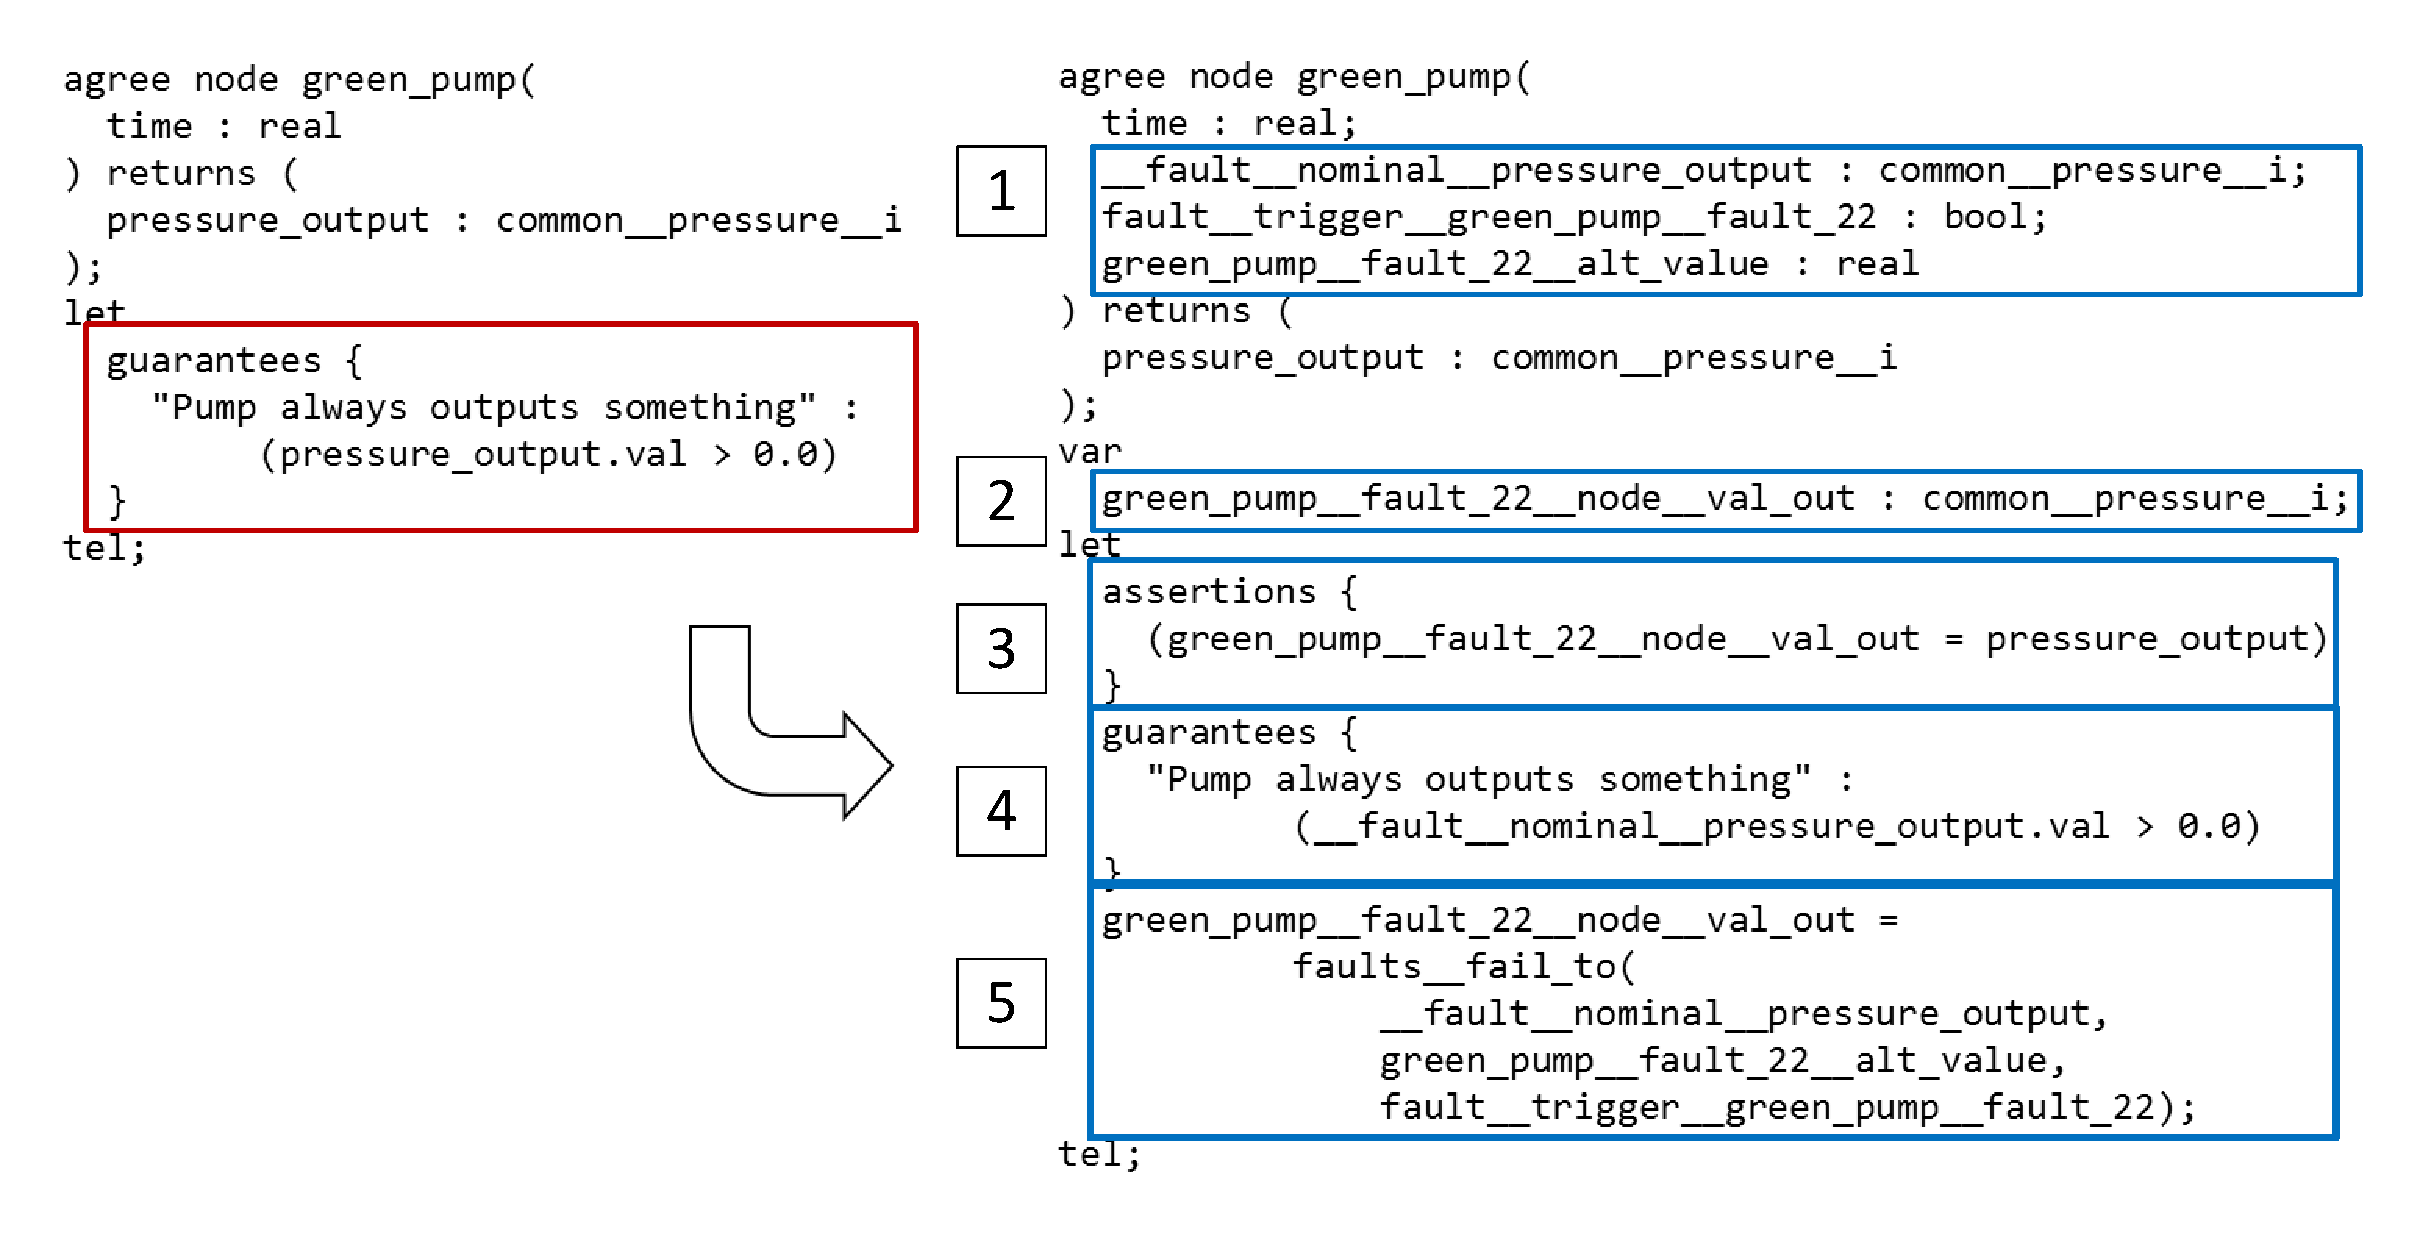
\includegraphics[trim=0 690 -10 70,clip,width=1.5\dimexpr\textwidth-2cm\relax]{images/lustre.pdf}
		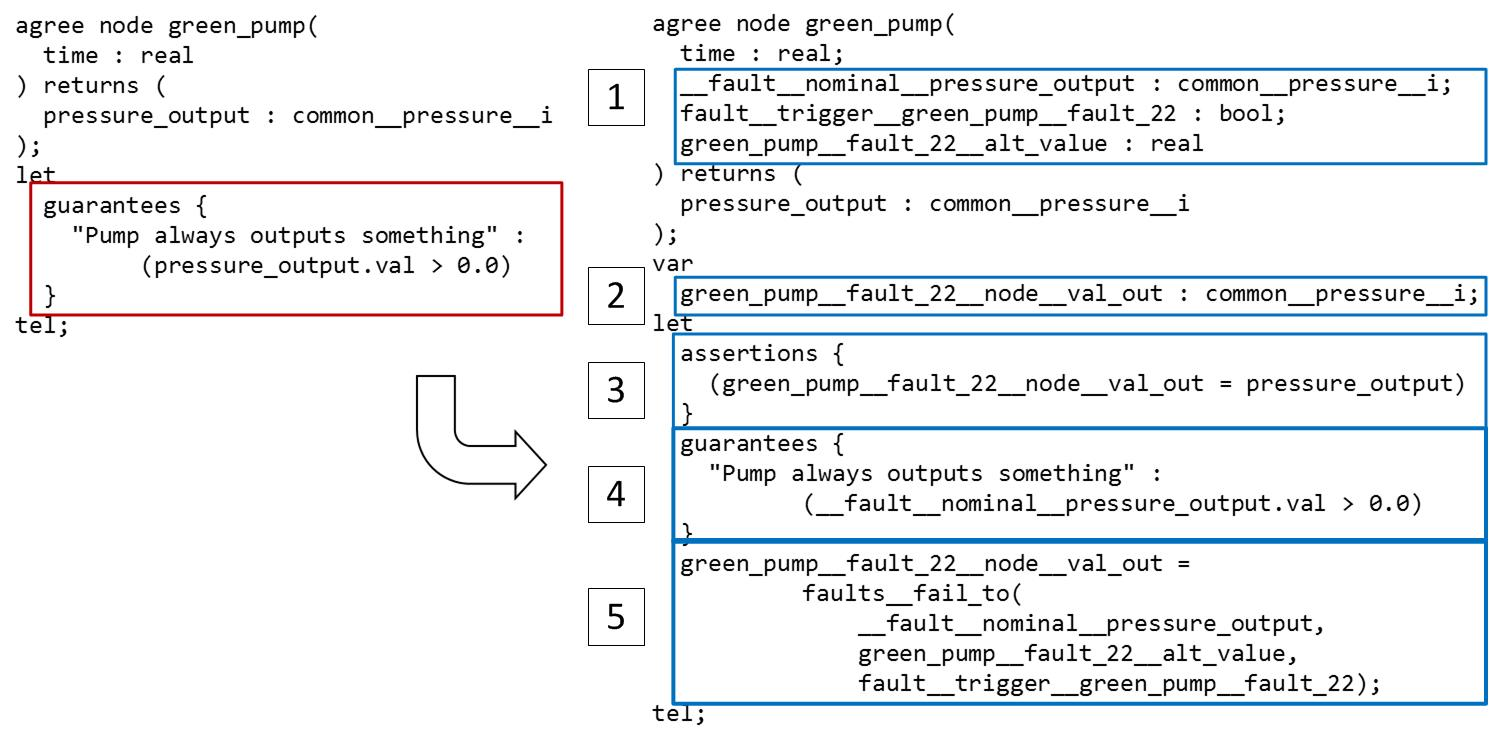
\includegraphics[scale=0.3]{images/lustre.jpg}
		\caption{Nominal AGREE node and its extension with faults}
		\label{fig:lustre}
	\end{center}
	\vspace{-0.3in}
\end{figure}

\begin{comment}
\begin{figure}
	\vspace{-0.1in}
	%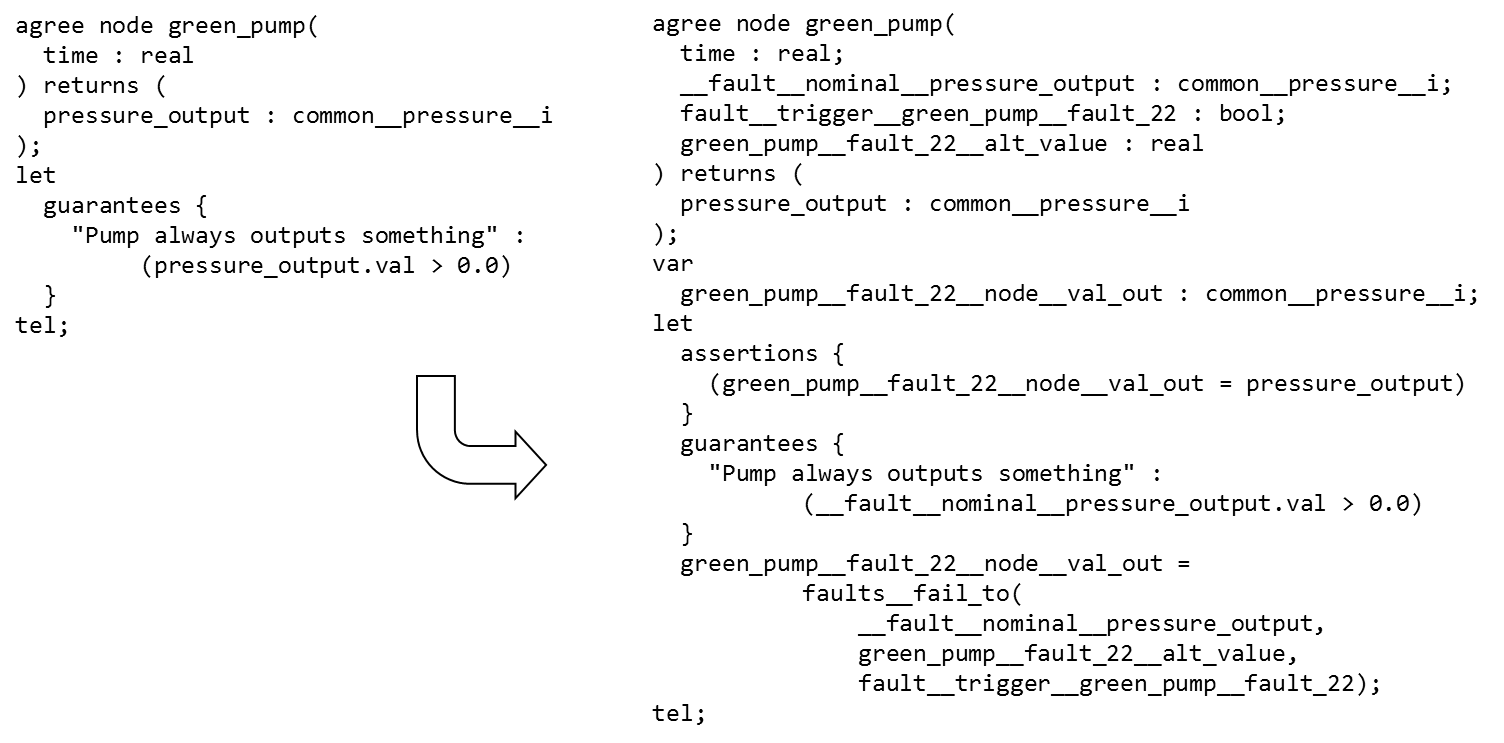
\includegraphics[trim=30 150 120 10,clip,width=\textwidth]{images/sample_code.png}
	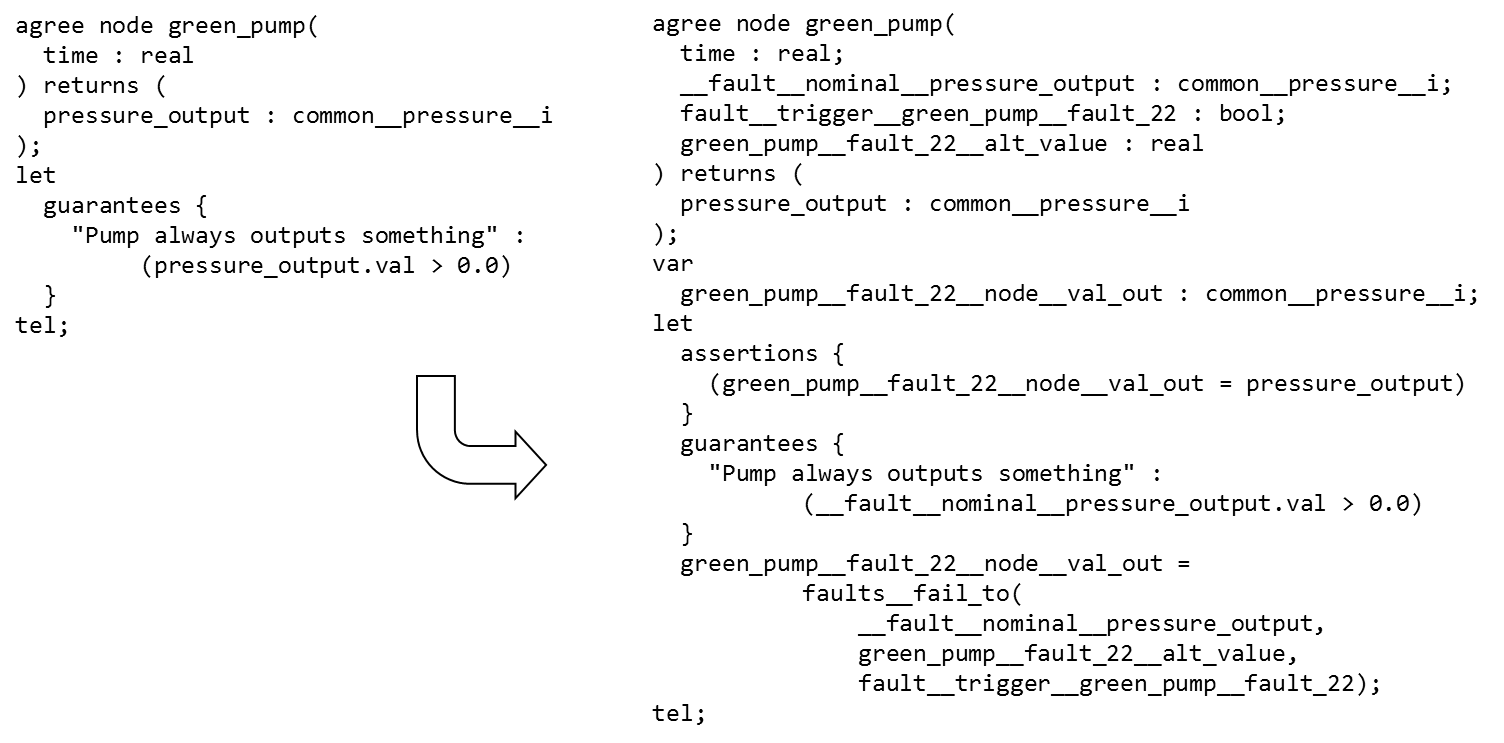
\includegraphics[width=\textwidth]{images/sample_code.png}
	\vspace{-0.3in}
	\caption{Nominal AGREE node and its extension with faults}
	\label{fig:comp}
\end{figure}
\end{comment}
%An annotation in the AADL model determines the fault hypothesis.  This may specify either a maximum number of faults that can be active at any point in execution (typically one or two), or that only faults whose probability of simultaneous occurrence is above some probability threshold should be considered. In the former case, we assert that the sum of the true {\em fault\_\_trigger} variables is below some integer threshold.  In the latter, we determine all combinations of faults whose probabilities are above the specified probability threshold, and describe this as a proposition over {\em fault\_\_trigger} variables.
%
%With the introduction of dependent faults, active faults are divided into two categories: independently active (activated by its own triggering event) and dependently active (activated when the faults they depend on become active). The top level fault hypothesis applies to independently active faults. Faulty behaviors augment nominal behaviors whenever their corresponding faults are active (either independently active or dependently active).

Once augmented with fault information, the AGREE model follows the standard translation path to the model checker JKind~\cite{2017arXiv171201222G}, an infinite-state model checker for safety properties.  The augmentation includes traceability information so that when counterexamples are displayed to users, the active faults for each component are visualized.


%For fault analysis, we separate the possible analyses available to users into two distinct actions and describe them here.


%\section{The Safety Annex}
\label{sec:detailed_approach}

In this section, we describe the main features and functionality of the Safety Annex. The usage of the terms error, failure, and fault follow their definitions in ARP4754A~\cite{SAE:ARP4754A}. We use {\em fault} as the generic modeling keyword throughout the AADL model hierarchy.

\subsection{Basic Functionality}

An AADL model of the nominal system behavior specifies the hardware and software components of the system and their interconnections. This nominal model is then annotated with assume-guarantee contracts using the AGREE annex~\cite{NFM2012:CoGaMiWhLaLu} for AADL. The nominal model requirements are verified using compositional verification techniques based on inductive model checking~\cite{2017arXiv171201222G}.

Once the nominal model behavior is defined and verified, the Safety Annex can be used to specify possible faulty behaviors for each component. The faults are defined on each of the relevant components using a customizable library of fault nodes and the faults are assigned a probability of occurrence. A probability threshold is also defined at the system level. This extended model can be analyzed to verify the behavior of the system in the presence of faults. Verification of the nominal model with or without the fault model is controlled through the safety analysis option during AGREE verification.

To illustrate the syntax of the Safety Annex, we use an example based on the Wheel Brake System (WBS) described in ~\cite{AIR6110} and used in our previous work ~\cite{Stewart17:IMBSA}.
The fault library contains commonly used fault node definitions. An example of a fault node is shown below:
\begin{figure}[h!]
	\hspace*{-4cm}
	\vspace{-0.5in} 
	\begin{center}
		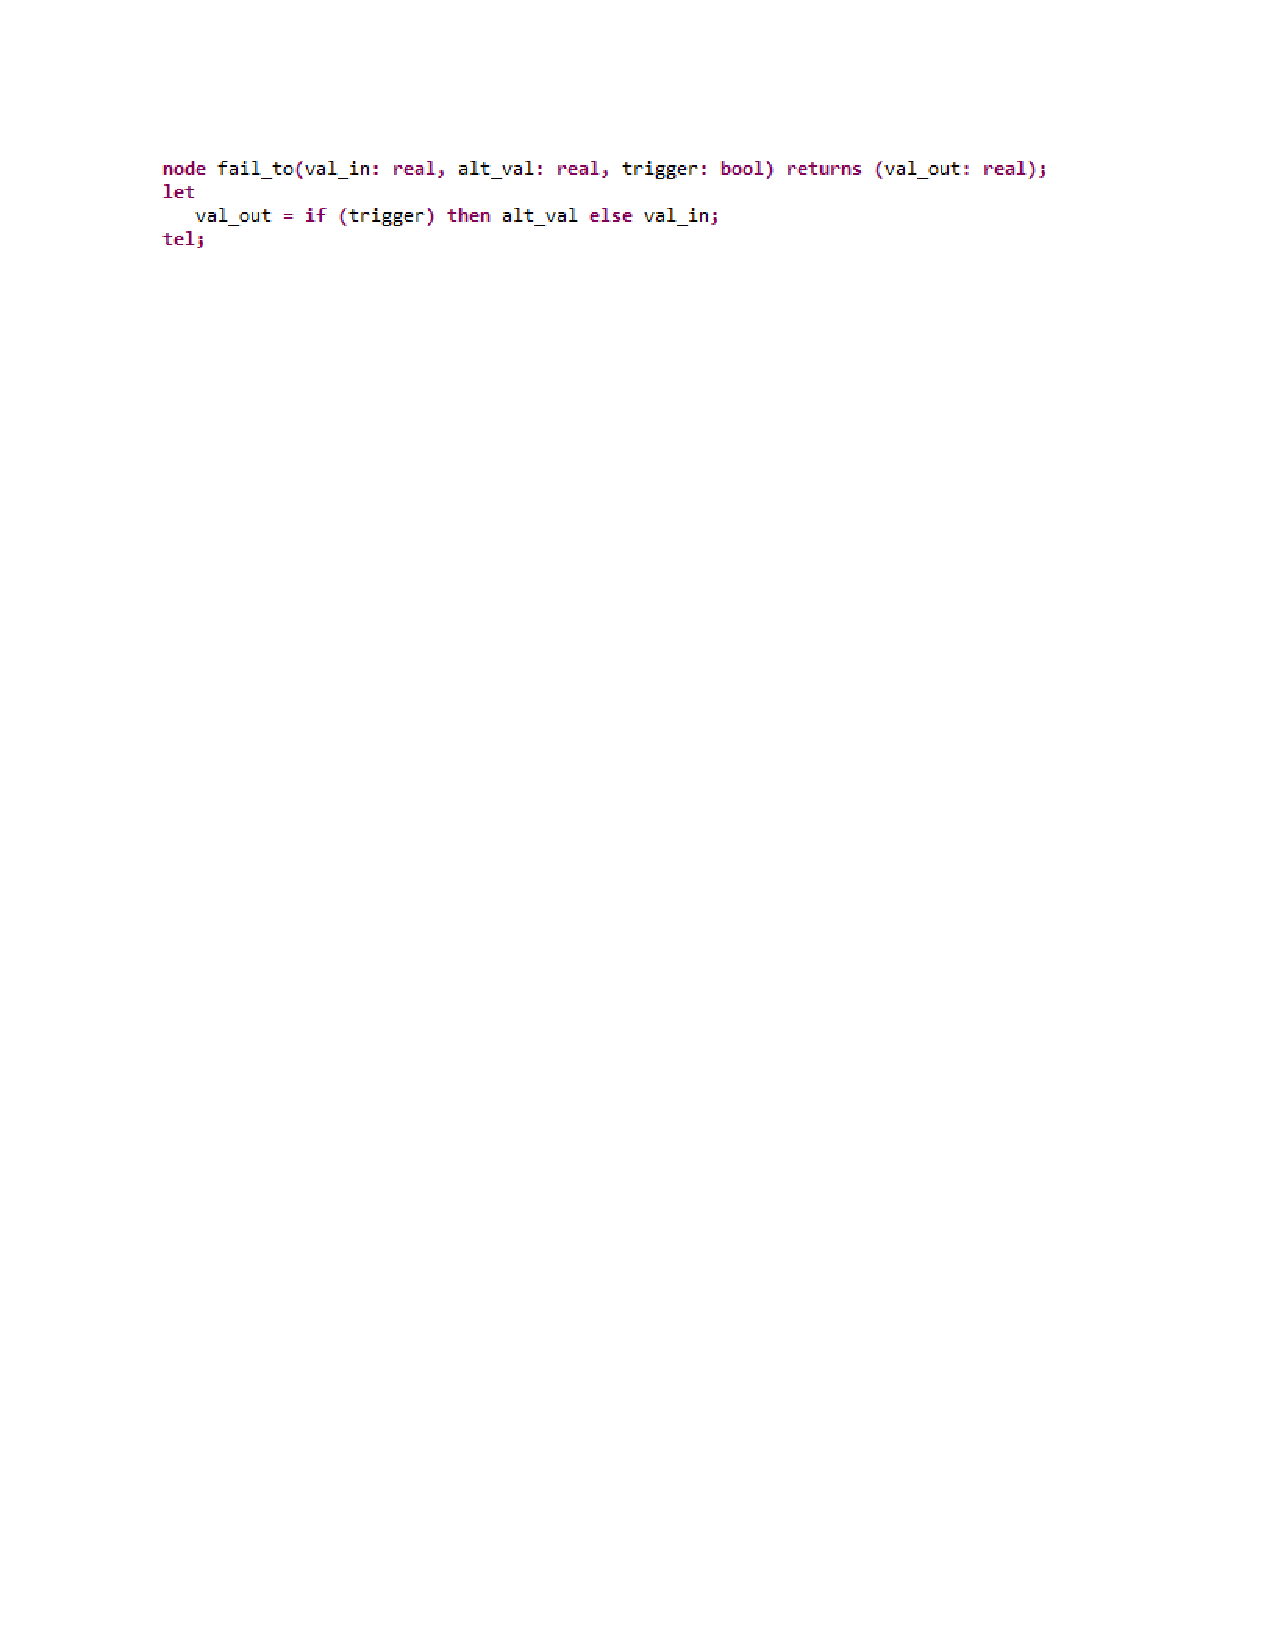
\includegraphics[trim=0 670 -10 70,clip,width=1.3\dimexpr\textwidth-1.5cm\relax]{images/fault_node.pdf}
	\end{center}
	\vspace{-0.4in}
\end{figure}

The \textit{fail\_to} node provides a way to inject a faulty input value. When the \textit{trigger} condition is satisfied, the nominal component output value is overridden by the \textit{fail\_to} failure value. In the WBS, the pump component generates an expected amount of pressure to a hydraulic line.  Declaration of a fail to zero fault in the pump component is shown below:
\begin{figure}[h!]
	\hspace*{-3cm} 
	\vspace{-0.6in}
	\begin{center}
		%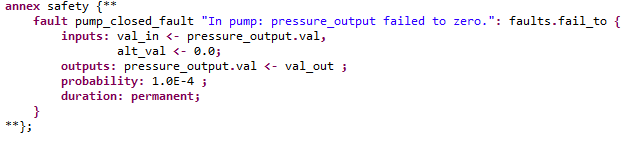
\includegraphics[trim=0 330 150 0,clip,width=1.0\textwidth]{images/pump_fault.png}
		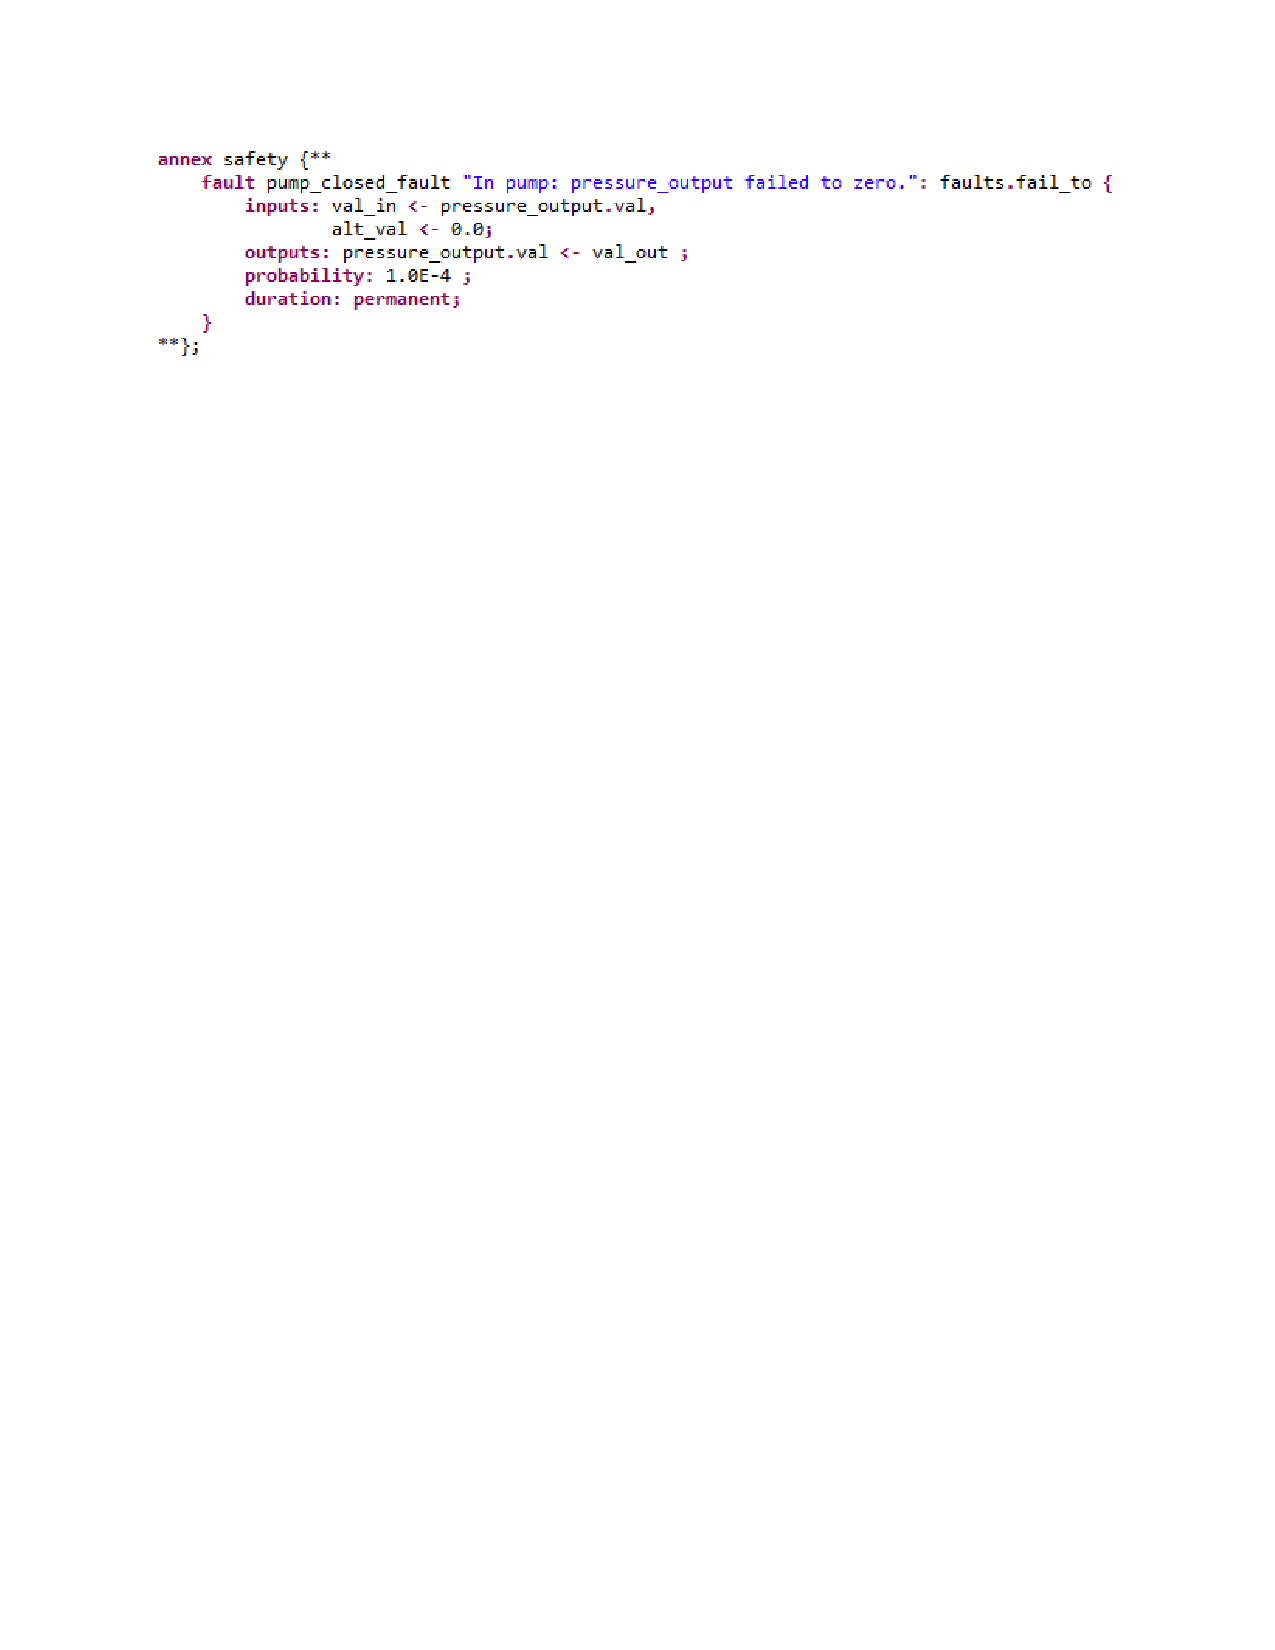
\includegraphics[trim=60 620 0 60,clip,width=1.3\dimexpr\textwidth-1.5cm\relax]{images/pump_fault.pdf}
	\end{center}
	\vspace{-0.40in}
\end{figure}

The \textit{fault statement} consists of a unique description string, the fault node definition name, and a series of \textit{fault subcomponent} statements. \\
\textbf{Inputs} in a fault statement are the parameters of the fault node definition. In the example above, \textit{val\_in} and \textit{alt\_val} are the two input parameters of the fault node. These are linked to the output from the Pump component (\textit{pressure\_output.val}), and \textit{alt\_value}, a fail to value of zero. When the analysis is run, these values are passed into the fault node definition.\\
\textbf{Outputs} of the fault definition correspond to the outputs of the fault node. The fault output statement links the component output (\textit{pressure\_output.val}) with the fault node output (\textit{val\_out}). If the fault is triggered, the nominal value of \textit{pressure\_output.val} is overridden by the failure value output by the fault node. Faulty outputs can take deterministic or non-deterministic values. \\
\textbf{Probability} (optional) describes the probability of a fault occurrence.\\
\textbf{Duration} describes the duration of the fault; currently the Safety Annex supports transient and permanent faults.\\
%\textit{Equation Statements}: Equation statements support deterministic or nondeterministic types. For more details on equation statements, see ~\cite{NFM2012:CoGaMiWhLaLu}.

\subsection{Hardware Failures and Dependent Faults}

Failures in hardware (HW) components can trigger behavioral faults in the software (SW) or system (SYS) components that depend on them.  For example, a CPU failure may trigger faulty behavior in threads bound to that CPU. In addition, a failure in one HW component may trigger failures in other HW components located nearby, such as cascading failure caused by a fire or water damage.

Faults propagate in AGREE as part of a system’s nominal behavior. This means that any propagation in the HW portion of an AADL model would have to be artificially modeled using data ports and AGREE behaviors in SW. This is less than ideal as there may not be concrete behaviors associated with HW components. In other words, faulty behaviors mainly manifest themselves on the SW/SYS components that depend on the hardware components.

To better model faults at the system level dependent on HW failures, we have introduced a new fault model element for HW components. In comparison to the basic fault statement introduced in the previous section, users are not specifying behavioral effects for the HW failures, nor data ports to apply the failure. An example of a model component fault declaration is shown below:
\begin{figure}[h!]
		\vspace{-0.2in}
	\begin{center}
		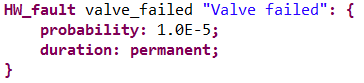
\includegraphics[width=.5\textwidth]{images/hw_fault.png}
	\end{center}
	\vspace{-0.4in}
\end{figure}

In addition, users specify fault dependencies/propagations outside of fault statements and inside safety annex, typically in the system implementation where the system configuration that causes the dependencies (e.g., binding between SW and HW components, co-location of HW components) becomes clear. This is because fault propagations are typically tied to the way components are connected or bound together; this information may not be available when faults are being specified for individual components. Having fault propagations specified outside of a component’s fault statements also makes it easier to reuse the component in different systems. An example of a fault dependency specification is shown below, showing that the valve{\_}failed fault at the shutoff subcomponent triggers the pressure{\_}fail{\_}blue fault at the selector subcomponent.
\begin{figure}[h!]
	\vspace{-0.2in}
	\begin{center}
		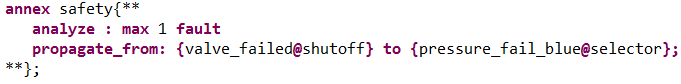
\includegraphics[width=.9\textwidth]{images/fault_propagation.png}
	\end{center}
	\vspace{-0.4in}
\end{figure}

\subsection{Architecture and Implementation}

The architecture of the Safety Annex is shown in Figure~\ref{fig:plugin-arch}.  It is written in Java as a plug-in for the OSATE AADL toolset, which is built on Eclipse.  It is not designed as a stand-alone extension of the language, but works with behavioral contracts specified in AGREE AADL annex and associated tools~\cite{NFM2012:CoGaMiWhLaLu}.  AGREE allows {\em assume-guarantee} behavioral contracts to be added to AADL components.  The language used for contract specification is based on the Lustre dataflow language~\cite{Halbwachs91:IEEE}. AGREE improves scalability of formal verification to large systems by decomposing the analysis of a complex system architecture into a collection of smaller verification tasks that correspond to the structure of the architecture.

\begin{figure}
	\begin{center}
		%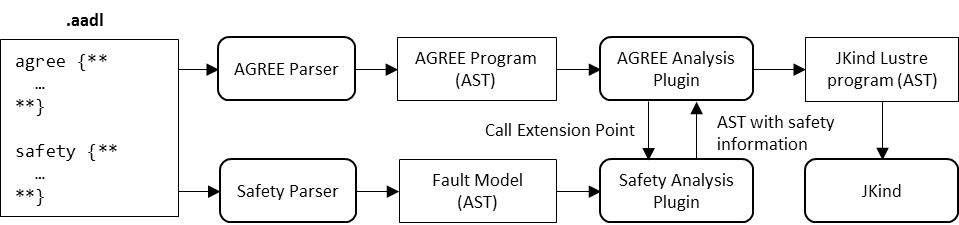
\includegraphics[trim=0 400 430 0,clip,width=0.85\textwidth]{images/arch.png}
		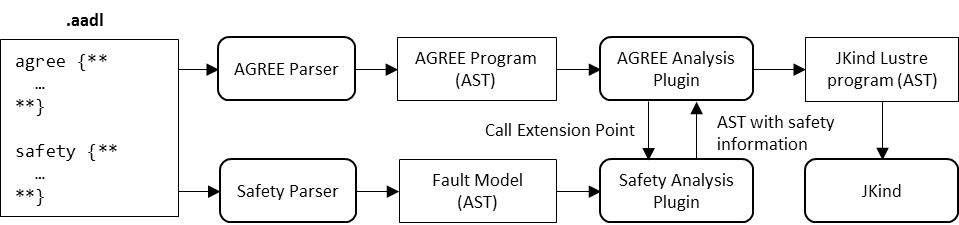
\includegraphics[width=.9\textwidth]{images/arch.png}
	\end{center}
	\vspace{-0.2in}
	\caption{Safety Annex Plug-in Architecture}
	\label{fig:plugin-arch}
\end{figure}

AGREE contracts are used to define the nominal behaviors of system components as {\em guarantees} that hold when {\em assumptions} about the values the component's environment are met.  The Safety Annex extends these contracts to allow faults to modify the behavior of component inputs and outputs.  To support these extensions, AGREE implements an Eclipse extension point interface that allows other plug-ins to modify the generated abstract syntax tree (AST) prior to its submission to the solver.  If the Safety Annex is enabled, these faults are added to the AGREE contract and, when triggered, override the nominal guarantees provided by the component.  An example of a portion of an initial AGREE node and its extended contract is shown in Figure~\ref{fig:comp}.  The \texttt{\_\_fault} variables and declarations are added to allow the contract to override the nominal behavioral constraints (provided by guarantees) on outputs.  In the Lustre language, \texttt{assertion}s are constraints that are assumed to hold in the transition system.

\begin{figure}
	\vspace{-0.1in}
	%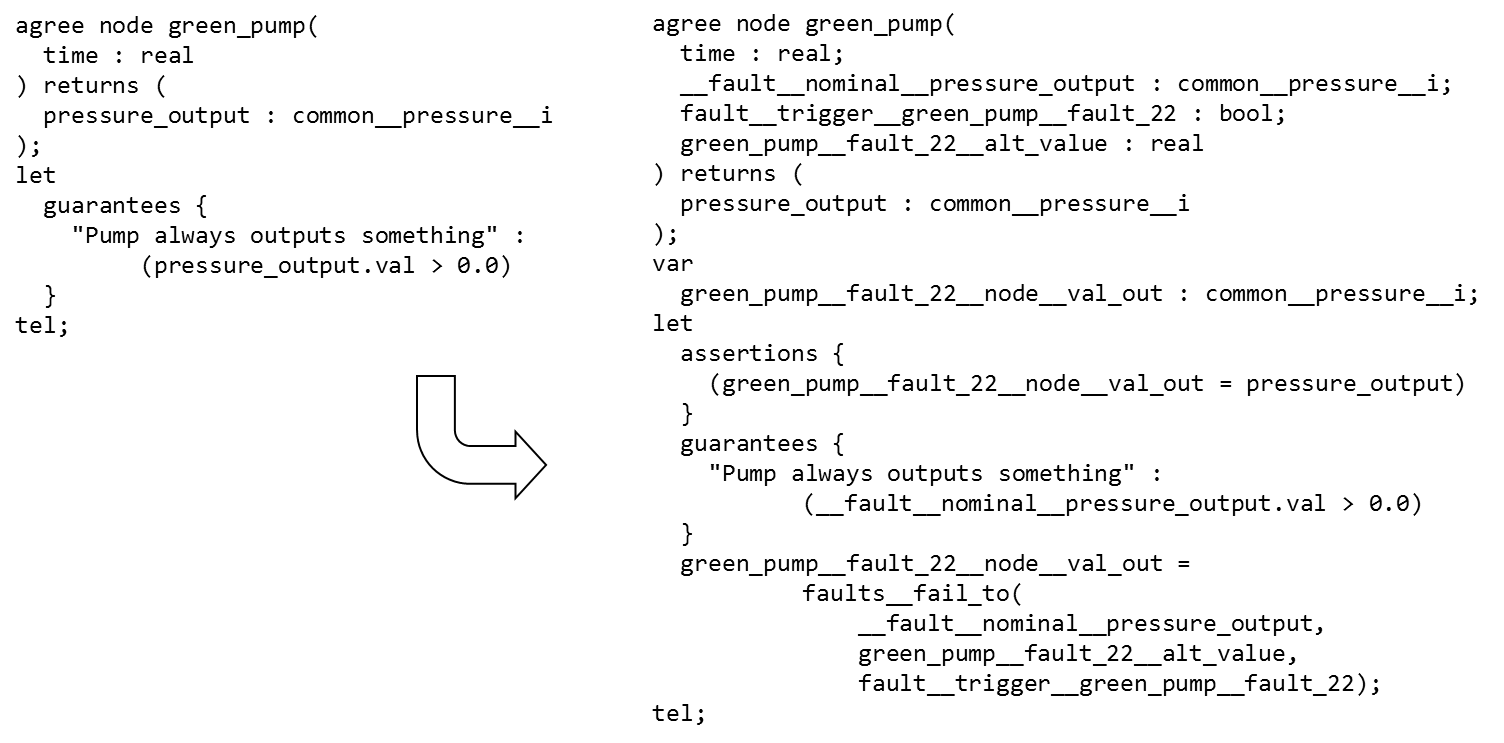
\includegraphics[trim=30 150 120 10,clip,width=\textwidth]{images/sample_code.png}
	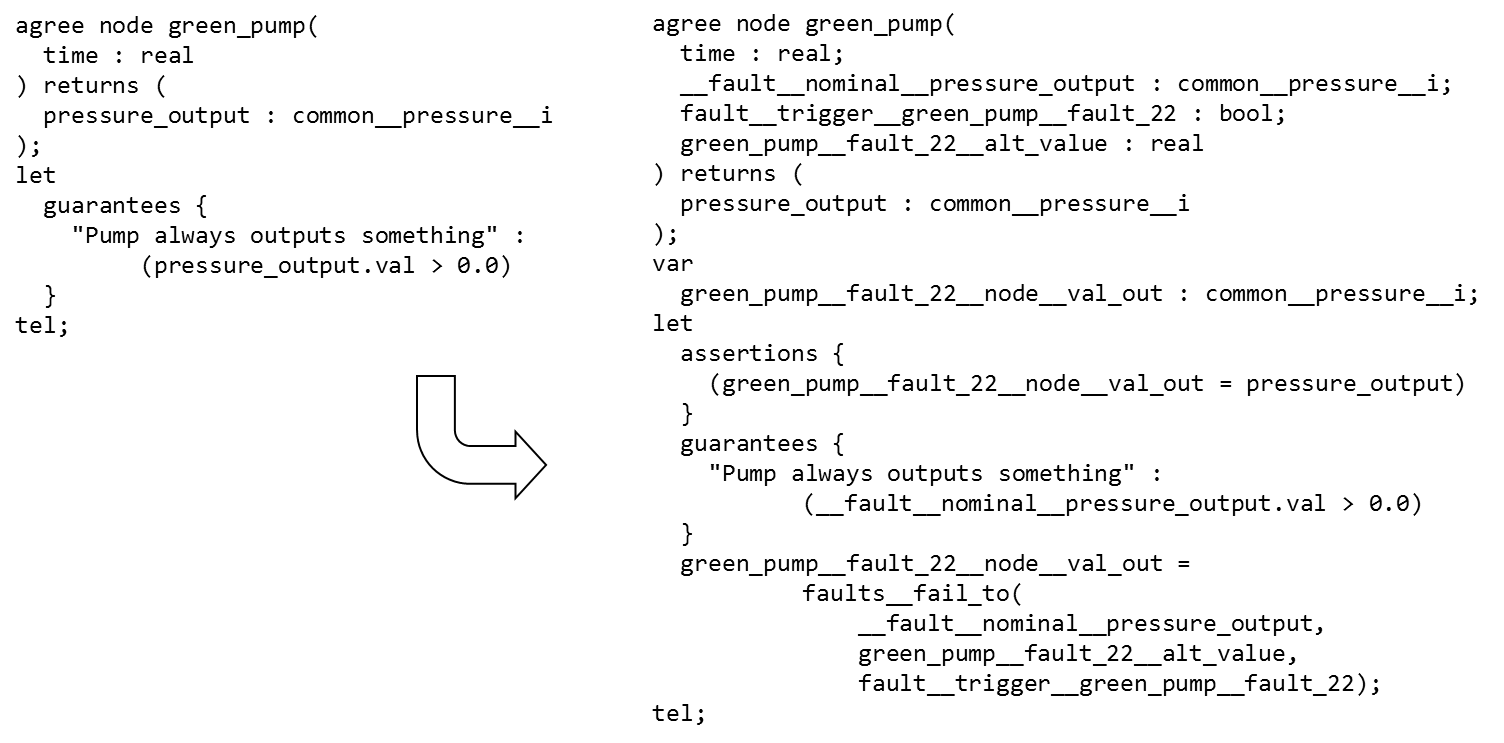
\includegraphics[width=\textwidth]{images/sample_code.png}
	\vspace{-0.3in}
	\caption{Nominal AGREE node and its extension with faults}
	\label{fig:comp}
\end{figure}

An annotation in the AADL model determines the fault hypothesis.  This may specify either a maximum number of faults that can be active at any point in execution (typically one or two), or that only faults whose probability of simultaneous occurrence is above some probability threshold should be considered. In the former case, we assert that the sum of the true {\em fault\_\_trigger} variables is below some integer threshold.  In the latter, we determine all combinations of faults whose probabilities are above the specified probability threshold, and describe this as a proposition over {\em fault\_\_trigger} variables.
%
With the introduction of dependent faults, active faults are divided into two categories: independently active (activated by its own triggering event) and dependently active (activated when the faults they depend on become active). The top level fault hypothesis applies to independently active faults. Faulty behaviors augment nominal behaviors whenever their corresponding faults are active (either independently active or dependently active).

Once augmented with fault information, the AGREE model follows the standard translation path to the model checker JKind~\cite{2017arXiv171201222G}, an infinite-state model checker for safety properties.  The augmentation includes traceability information so that when counterexamples are displayed to users, the active faults for each component are visualized.


%\subsection{Mapping to Safety Analysis Artifacts}

\begin{comment}
The following list describes how the basic safety concepts can be represented using the Safety Annex.

\begin{enumerate}
\item \textbf{Error} Definition and how we model it
\item \textbf{Fault} Definition and how we model it
\item \textbf{Failure} Definition and how we model it. Non deterministic faults
\item \textbf{Failure Mode}
\end{enumerate}


Errors/Faults/Failures - to a safety engineer, these terms have very specific meanings.  You will see my specific comments on this topic where I located them by your Section 3.3.  If needed, we can talk about this comment after I send you my mark-ups.
In Section 3.1, you introduce the term "non-deterministic".  I am not sure how your new process can be used by the safety engineering discipline unless things are "deterministic" and therefore "repeatable".
\end{comment}

\begin{comment}
A prerequisite of performing the safety assessment of a system design is to understand how the system works, primarily focusing on the integrity of the outputs and the availability of the product. The safety engineers then use the acquired understanding to conduct safety analysis, construct the safety analysis artifacts, and compare the analysis results with established safety objectives and safety related requirements.
%check Figure 7 of ARP-4754A for step by step process of the traditional approach
%How our approach can help: step by step process; inputs and outputs
%Drawback/inefficiencies with the current safety assessment
%The causal effect in the fault tree is manually come up by safety engineers after understanding the signal and function flow in the system/sw design documents for the related functionality.
%The logical causal relationship is represented in a descriptive fault tree structure.
%It works well when the signals are processed in a sequential/linear fashion, but not when there are interactions/feedback loops that make the causal effect no longer linear?

%case study
%AIR6110, Rockwell white paper
"working on safety analysis process. Strategy:
1. Check the example Mike Peterson did with stall warning
2. Come up with model in our end
3. See if we can catch anything missed by the fault tree, or help supply the fault tree analysis"
start process investigation by:
1. select the example from stall warning where mike has produced a fault tree from the document
2. independently model from the stall warning doc and try to:
get information from the fault tree that can build the structure of the fault tree
get information from the verification that can help trim/update the probability numbers of the fault tree
3. Compare the fault tree produced by Mike and the information supplied by our study, and see if we provide values to this study
Repeat this for an example fault tree from the white paper Mike sent

Process investigation
How should our model interact with the fault tree that Mike come up with? Any place we can work to create the tree for him? Or provide additional scenarios? Or validate the probabilities for his tree? Or SW/HW/Sys interactions that our approach captures that is hard to capture/verify using his approach?
How does the behavioral/interaction part of the document be modeled in the fault tree and in our model?
What findings from the safety process is driving the model/design updates, such as redundancy?
Would the AMASE modeling and analysis approach justify to make a conservative fault tree less conservative?
How the process steps are different from the process steps for ARP4761A MBSA?

With our process, do we have to use our tool/approach? Or other tools/approaches like xSAP could also work? What's the uniqueness of using our tool in this process? What's the benefit of this process in comparison to the current/traditional safety process?

"Documents to read:
- the white paper by Mike Peterson's group
- ARP4761A model based development supplement
- AIR 6110
- ARP4761
- ARP4754"
According to ARP4761A MBSA supplement draft, the MBSA model is called the Failure Propagation Model (FPM).
ARP4761A MBSA supplement identified some limitation of MBSA, including "it may be difficult to represent complicated Failed Conditions".
Check the simple example (Section 6) in ARP4761A MBSA

Answer from process point of view: why is our approach better than what's out there? What problem are we trying to solve?
Are we doing FPM (Failure Propagation Model) per ARP4761 MBSA?
MBSA section 6.2 shows a complex MBSA example

Give a detailed description of how fault tree is related to the AMASE nominal and faulty model, and the results from the AMASE verificaiton is relayed/fed bak to the fault tree
\end{comment}


% \section{Case Studies}
\label{sec:case_study}
To demonstrate the effectiveness of the Safety Annex, we describe two case studies.



\iffalse
\subsection{Simple Wheel Brake System}
The Wheel Brake System (WBS) described in ARP4761 has been used as a case study for safety analysis, formal verification, and contract based design in numerous studies. In order to show scalability compare results with other tools and studies, the AADL model of the WBS used in~\cite{Stewart17:IMBSA} was enhanced using as a guide the NuSMV ARCH4 model as described in~\cite{DBLP:conf/cav/BozzanoCPJKPRT15}. This version of the WBS model was chosen due to the complexity of the model and because this model addresses required safety concerns (for description of these concerns, see~\cite{DBLP:conf/cav/BozzanoCPJKPRT15}). Due to the added complexity of this WBS system, a short description of the subcomponents and behavior is necessary.

\subsubsection{Simple WBS architecture description}
The highest level model component is the WBS. It consists of the Braking System Control Unit (BSCU), green and blue hydraulic pressure lines (supplied by the green and blue hydraulic pumps respectively), a selector which selects between normal operating mode and alternate operating mode, and the wheel system.

There are three operating modes of the WBS. In \textit{normal} mode, the system uses the \textit{green} hydraulic circuit. In \textit{alternate} mode, the system uses the \textit{blue} hydraulic circuit.  If the BSCU detects lack of pressure from the green line or one of its command units are invalid, then the system switches into alternate mode. The last mode of operation of the WBS is the \textit{emergency} mode. This is supported by the blue circuit but operates if the blue hydraulic pump fails. The accumulator pump has a reserve of pressurized hydraulic fluid and will supply this to the blue circuit in emergency mode.  Antiskid braking commands receive data from the BSCU that will determine if skidding is found at the wheel and handle accordingly.

In the simplified WBS model, there is one wheel that receives pressure from either the green or blue line. This wheel provides feedback to the BSCU providing information about the pressure supplied.

To evaluate the effectiveness of the Safety Annex, we updated the simple WBS model~\cite{Stewart17:IMBSA} to specify faulty component behaviors. The components' nominal  and faulty behaviors are modeled separately. At the top-level AADL component, the fault hypothesis was specified as the maximum number of faults that can be active at any time. The AGREE contracts at the top-level component were verified using AGREE, with the ``Perform Safety Analysis'' option selected. This signals the tool to weave the nominal and faulty behaviors into one augmented AGREE model before feeding to the model checker.

In this example, the top level contract ``Pedal pressed and no skid implies brake pressure applied'' was verified in the presence of at most one fault active during execution.  However, it was shown to be invalid when more than one fault was allowed. The counterexample indicated that both Selector's outputs failed to non-deterministic values due to the faults introduced.
\fi


\subsection{Wheel Brake System}
%original in the case study:
%The Wheel Brake System (WBS) described in ARP4761 has been used as a case study for safety analysis, formal verification, and contract based design in numerous studies. In order to show scalability compare results with other tools and studies, the AADL model of the WBS used in~\cite{Stewart17:IMBSA} was enhanced using as a guide the NuSMV ARCH4 model as described in~\cite{DBLP:conf/cav/BozzanoCPJKPRT15}. This version of the WBS model was chosen due to the complexity of the model and because this model addresses required safety concerns (for description of these concerns, see~\cite{DBLP:conf/cav/BozzanoCPJKPRT15}). Due to the added complexity of this WBS system, we provide a short description of the subcomponents and behavior.
%from related work:
%The Wheel Brake System (WBS) described in ARP4761~\cite{SAE:ARP4761} has been used in the past as a case study for safety analysis, formal verification, and contract based design~\cite{DBLP:conf/cav/BozzanoCPJKPRT15, 10.1007/978-3-319-11936-6-7, CAV2015:BoCiGrMa, Stewart17:IMBSA, propBasedProofSys, Joshi05:SafeComp, NasaRep:MBSA-Aug05} The preliminary work for the safety annex used a simplified model of the WBS~\cite{Stewart17:IMBSA}. In order to show scalability and compare results with other studies, an AADL version of the WBS was designed based off of arch4wbs NuSMV model described in previous work~\cite{DBLP:conf/cav/BozzanoCPJKPRT15}. This model was chosen due to the number of subcomponents in the system and the complexity of behavior captured in the NuSMV model.

The Wheel Brake System (WBS) described in ARP4761~\cite{SAE:ARP4761} has been used in the past as a case study for safety analysis, formal verification, and contract based design~\cite{DBLP:conf/cav/BozzanoCPJKPRT15, 10.1007/978-3-319-11936-6-7, CAV2015:BoCiGrMa, Stewart17:IMBSA, propBasedProofSys, Joshi05:SafeComp, NasaRep:MBSA-Aug05}. The preliminary work for the safety annex used a simplified model of the WBS~\cite{Stewart17:IMBSA}. In order to demonstrate scalability of our tools and compare results with other studies, we constructed a functionally and structurally equivalent AADL version of %most complex 
\janet{the more complex} WBS NuSMV model (arch4wbs) described in previous work~\cite{DBLP:conf/cav/BozzanoCPJKPRT15}.  %It was chosen due to the complexity of the model and because this model addresses required safety concerns (for description of these concerns, see~\cite{DBLP:conf/cav/BozzanoCPJKPRT15}). 
We describe the elaborations of this model to the ARP4761 WBS below.
%Due to the added complexity of this WBS system, we provide a short description of the subcomponents and behavior.

\subsubsection{WBS architecture description}
The WBS is composed of two main systems: the control system and the physical system. The control system electronically controls the physical system and contains a redundant Braking System Control Unit (BSCU) in case of failure. The physical system consists of the hydraulic circuits running from hydraulic pumps to wheel brakes. This is what provides braking force to each of the 8 wheels of the aircraft.

There are three operating modes in the WBS model. In \textit{normal} mode, the system uses the \textit{green} hydraulic circuit. The normal system is composed of the green hydraulic pump and one meter valve per each of the 8 wheels. Each of the 8 meter valves are controlled through electronic commands coming from the BSCU. These signals provide brake commands as well as antiskid commands for each of the wheels. The braking command is determined through a sensor on the pilot pedal position. The antiskid command is calculated based on information regarding ground speed, wheel rolling status, and braking commands.

In \textit{alternate} mode, the system uses the \textit{blue} hydraulic circuit.  The wheels are all mechanically braked in pairs (one pair per landing gear). The alternate system is composed of the blue hydraulic pump, four meter valves, and four antiskid shutoff valves. The meter valves are mechanically commanded through the pilot pedal corresponding to each landing gear. If the system detects lack of pressure in the green circuit, the selector valve switches to the blue circuit. This can occur if there is a lack of pressure from the green hydraulic pump, if the green hydraulic pump circuit fails, or if pressure is cut off by a shutoff valve. If the BSCU unit becomes invalid, the shutoff valve is closed.

The last mode of operation of the WBS is the \textit{emergency} mode. This is supported by the blue circuit but operates if the blue hydraulic pump fails. The accumulator pump has a reserve of pressurized hydraulic fluid and will supply this to the blue circuit in emergency mode.

The model, which is available at \mike{Where is model?}, has substantial complexity \janet{another word for ``substantial''?}. It contains 30 different kinds of components, 169 component instances, a model nesting depth of 5 levels (an AADL system is decomposed into other systems, which are further decomposed, up to a depth of 5 levels).  The total model involves 17 assumptions and 113 guarantees, with 11 top-level system properties.  There are a total of 33 different fault types and 141 fault instances within the model.  The large number of fault instances is due to the redundancy in the model and the use of 8 wheels.

\mike{An example property would be very useful here!}



\subsubsection{Fault Analysis of WBS using Safety Annex}

\iffalse
%After the verification was completed, we defined faults equivalent to those described in the xSAP model for the NuSMV WBS system in~\cite{DBLP:conf/cav/BozzanoCPJKPRT15}. 

\begin{figure}[h!]
	\vspace{-0.17in}
	\begin{center}
		%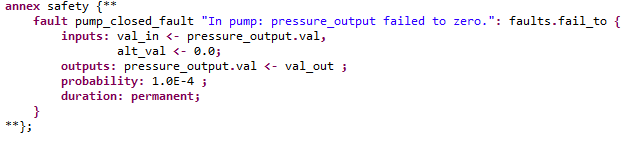
\includegraphics[trim=0 330 150 0,clip,width=1.0\textwidth]{images/pump_fault.png}
		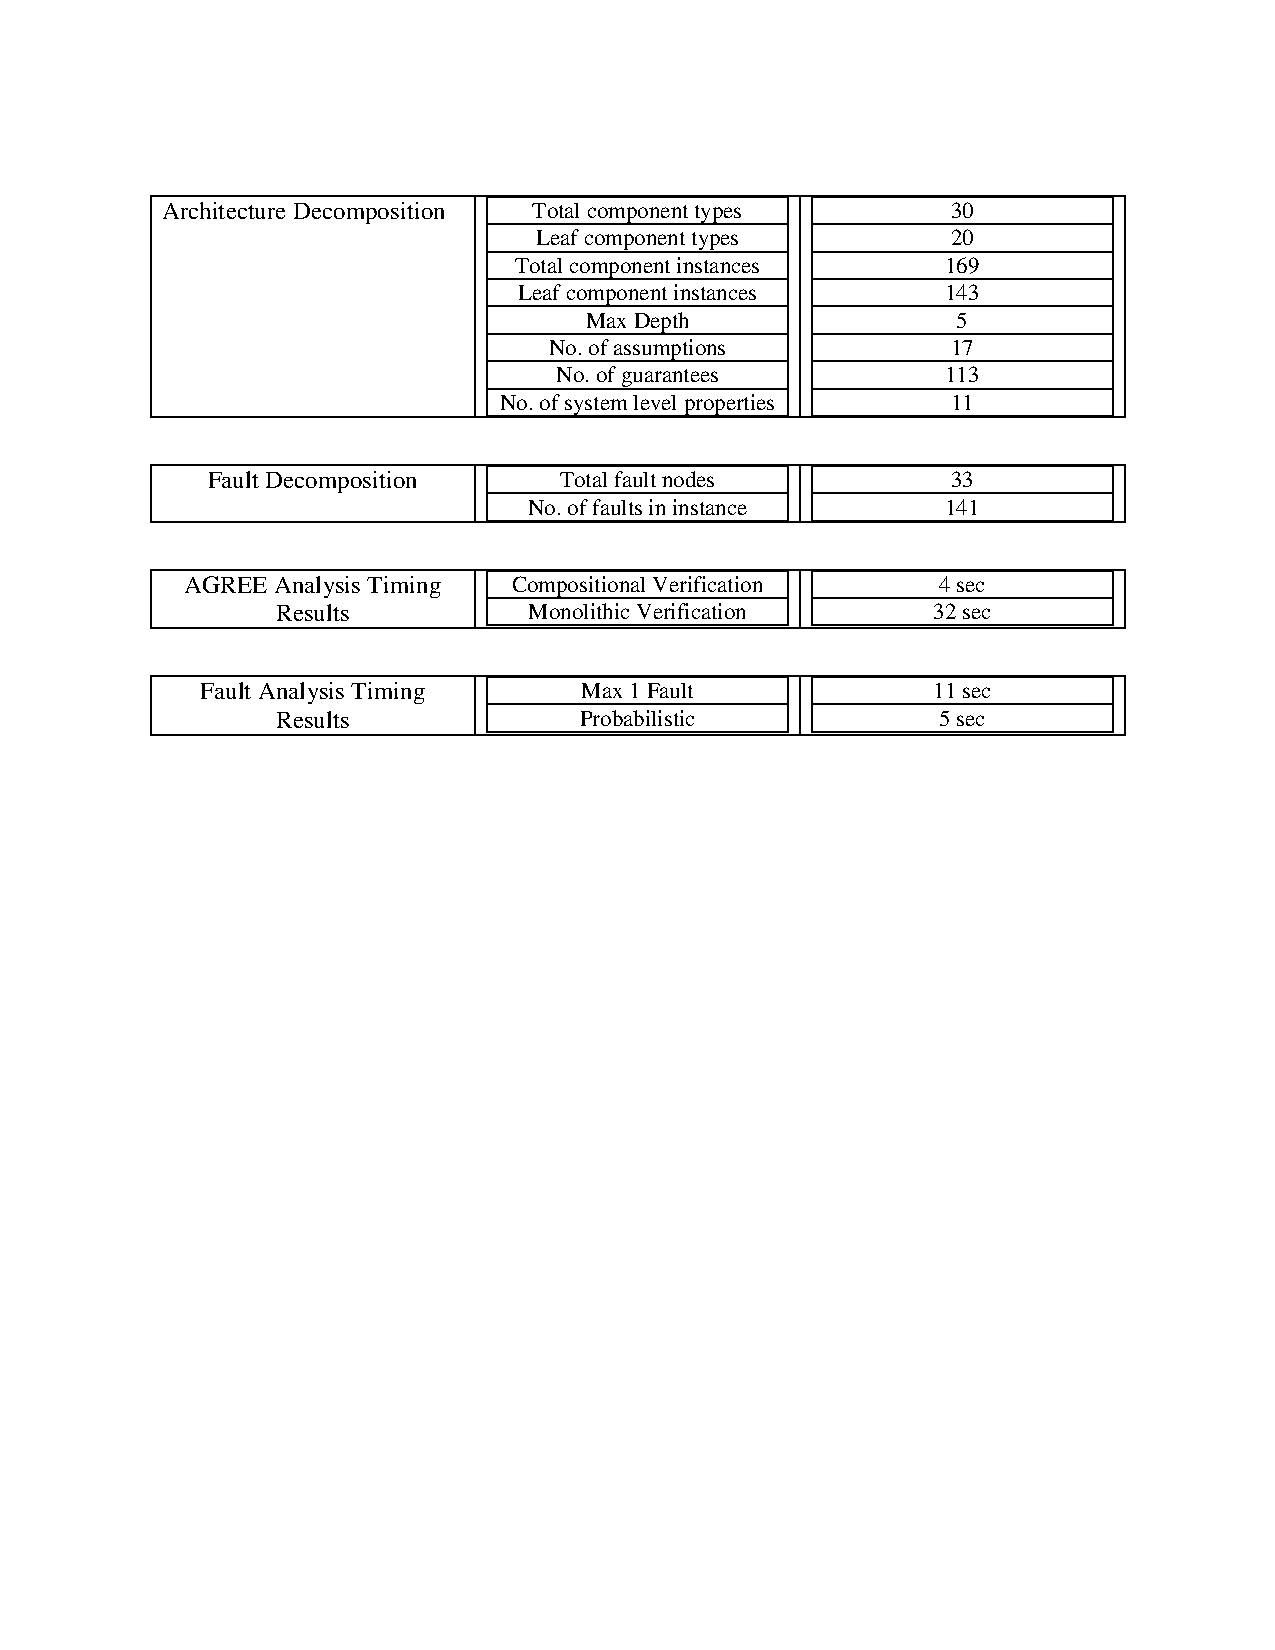
\includegraphics[trim=0 435 0 90,clip,width=1.0\textwidth]{images/arch_table.pdf}
		\caption{Modeling, Verification, and Fault Analysis Metrics}
 		\label{fig:metrics}
	\end{center}
	\vspace{-0.40in}
\end{figure}
\fi 


Fault analysis on the top level WBS system was performed on 11 top-level properties using two fault hypotheses: the first allows at most one fault and the second allows combinations of faults that exceed the acceptable probabilities for the top-level hazard defined in ARP4761~\cite{SAE:ARP4761}.

We examine scalability by looking at analysis times for both compositional verification, where the verification task is split into layers to be analyzed separately, and monolithic verification, where the entire system is analyzed in one pass.  When considering the nominal system behavior (no faults), the total time required for analysis using compositional verification is \mike{What is the aggregate time?}, and the time for monolithic analysis is 32 seconds.  This nominal model is too small to gain significant benefit from compositional analysis.  However, when we consider faulty behavior, when given a single-fault hypothesis, the total time for compositional analysis is X \mike{what is X?}, and the time for monolithic analysis is Y \mike{what is Y?}, clearly demonstrating the value of compositional analysis for more complex models.  Similarly, for probabilistic analysis, the compositional time is \mike{Z} and the monolithic time is \mike{A}.

In our analysis, we discovered that most properties pass the model, but the \textit{Inadvertant braking at the wheel} properties were not resilient to a single fault nor did they meet the desired $10^{-9}$ fault threshold for probabilistic analysis.  In our model (as in the NuSMV model~\cite{DBLP:conf/cav/BozzanoCPJKPRT15}, there is a single pedal position sensor for the brake pedal.  If this sensor fails, it can command braking without a pilot request.  It was straightforward for us to diagnose the cause of the property failure using an automatically generated {\em counterexample}, which is a test case that demonstrates the failure.  

This counterexample can be used to further iterate system design.  For our model, it could be that the time in the V1 phase of flight is short enough that we need to adjust our model failure rates for the V1 time scale, or that redundant sensors are required on the pedals (here we note that the architecture of the pedal assembly is not discussed in ARP4761).  It is straightforward and computationally inexpensive to run the analysis, allowing quick iterations between systems and safety engineers. \janet{As indicated in Figure~\ref{fig:interaction_with_FTA}, the sync and update between the preliminary system FTA and the architecture/analysis model continues until the system safety property is satisfied with the desired fault tolerance and failure probability achieved.}

%In terms of the safety analysis process, this corresponds with an update in the preliminary system FTA which will eventually change the system FTA and impact SSA results.\mike{keep last sentence?}

%Mike: with regard to the safety process sentence at the end of the WBS case study, he thinks that we can keep that sentence, but update it to mention that we can iteratively run analysis if we don't achieve the desired fault tolerance for single failure or achieve the desired probability


\subsection{Quad-Redundant Flight Control System}
In order to discuss Byzantine faults and hardware failures with their propagations, we applied the Safety Annex to the Quad-Redundant Flight Control System (QFCS) model~\cite{QFCS15:backes}. Faulty behaviors were introduced in order to see the response of the system to several faults, and to evaluate fault mitigation logic in the model. The QFCS system-level properties failed when unhandled faulty behaviors were introduced.

We also used the Safety Annex to explore more complicated faults at the system level on a simplified QFCS model with cross-channel communication between its Flight Control Computers.

\begin{itemize}
	\item Byzantine faults~\cite{Driscoll-Byzantine-Fault} were simulated by creating one-to-one connections from the source to multiple observers so that disagreements could be introduced by injecting faults on individual outputs. \janet{The system level property ``at most one flight control computer in command'' was verified false in one second in the presence of Byzantine fault on the baseline model. The same property was verified true in three seconds on the model with Byzantine fault handling protocol implemented. System designers can use this approach to verify if a system design is resilient to Byzantine faults, examine vulnerabilities, and test if a mitigation mechanism works.} 

%original wording:	
	% A system-level property failed due to the fault on the baseline model, but did not fail on the model with Byzantine fault handling protocol added. Using the Safety Annex like this can test a system's vulnerability to Byzantine faults and verify mitigation mechanisms.
	
	\item Dependent faults were modeled by first injecting failures \janet{to the cross-channel data link (CCDL) bus (physical layer), and faults to the flight control computer (FCC) outputs (logical layer), then specifying fault propagations in the top level system implementation (where the data connections between FCC outputs were bound to the CCDL bus subcomponents). The fault propagation indicates that one CCDL bus failure can trigger all FCC output faults. With the fault hypothesis that maximum one fault active during execution, the system level property ``not all FCCs fail at the same time'' was verified false in one second.}
	 
%original wording:
%Dependent faults were modeled by injecting failures to hardware components (physical layer), and faults to software components (logical layer) that are bound to the hardware components, then specifying fault propagations at the QFCS system level to indicate that the software faults are dependent on the hardware failures. 	 
\end{itemize}

%\mike{Results?} \janet{updated the last two paragraphs}


%\section{Analysis of the Fault Model}
\label{sec:fault_analysis}

When the Safety Annex is enabled, users can invoke either the monolithic analysis or compositional analysis in AGREE to check if the top level safety properties of the system hold in the presence of faults under the fault hypothesis given for the system. If an active fault causes the violation of a contract, a counterexample is provided by the model checker. The counterexample can be used to further analyze the system design and make necessary updates to the shared model between safety assessment and system development processes. This iterations continues until the system safety property is satisfied with the desired fault tolerance and failure probability achieved.

\subsection{Fault Hypothesis}
As the number of component faults increases, the different fault combinations can grow exponentially, making model checking infeasible. Therefore, a fault hypothesis needs to be specified for the system under verification to limit the simultaneous fault activations that are considered by the model checker.

A Safety Annex annotation in the system implementation of the AADL model determines the fault hypothesis. There are two types of fault hypothesis:

The \textit{max fault hypothesis} specifies a maximum number of faults that can be active at any point in execution. This is analogous to restricting the cutsets to a specified maximum number of terms in the fault tree analysis in
traditional safety analysis. In implementation (i.e., the translated Lustre model feeding into the model checker), we assert that the sum of the true {\em fault\_\_trigger} variables is below some integer threshold. Each layer of the model needs to have a max fault hypothesis statement specified in order to consider fault activation in that layer in the analysis.

The \textit{probabilistic fault hypothesis} specifies that only faults whose probability of simultaneous occurrence is above some probability threshold should be considered (see Figure~\ref{fig:hwFaultProp}). This is analogous to restricting the cutsets to only those whose probability is above some set value. In implementation, we determine all combinations of faults whose probabilities are above the specified probability threshold and describe this as a proposition over {\em fault\_\_trigger} variables. Each subcomponent fault needs to specify a probability of occurrence in order to be considered in the analysis.

With the introduction of dependent faults, active faults are divided into two categories: independently active (activated by its own triggering event) and dependently active (activated when the faults they depend on become active). The top level fault hypothesis applies to independently active faults. Faulty behaviors augment nominal behaviors whenever their corresponding faults are active (either independently active or dependently active).

\subsection{Monolithic Analysis}
When monolithic analysis is performed on the nominal system model, the architectural model is flattened in order to perform the analysis. All of the contracts in the lower levels are used for the analysis.
%A top level threshold is defined within the safety annex located in the top level system implementation. In the lower levels, each defined subcomponent fault is given a probability of occurrence. 

Given a probabilistic fault hypothesis, this corresponds to performing a %prior 
analysis on which combinations of faults have a probability less than the threshold and then inserting assertions into the Lustre code accordingly. If the probability of such combination of faults is in fact less than the designated top level threshold, these faults may be activated and the behavioral effects can be seen through a counterexample.  

To perform this analysis, it is assumed that the non-hardware faults occur independently and possible combinations of faults are computed and passed to the Lustre model to be checked by the model checker. As seen in Algorithm 1, the computation first removes all faults from consideration that are too unlikely given the probability threshold. The remaining faults are arranged in a priority queue $\mathcal{Q}$ from high to low. Assuming independence in the set of faults, we take a fault with highest probability from the queue (step 5) and attempt to combine the remainder of the faults in $\mathcal{R}$ (step 7). If this combination is lower than the threshold (step 8), then we do not take into consideration this set of faults and instead remove the tail of the remaining faults in $\mathcal{R}$. %The reason we can do this is because of the arrangement in priority queue from highest to lowest value. If this combination is below threshold, certainly any other combination of these faults with one of lesser value in the priority queue will also be below threshold. 
 
In this calculation, we assume independence among the faults, but in the Safety Annex it is possible to define dependence between faults using a %\textit{hardware fault} node\
fault propagation statement. After fault combinations are computed using Algorithm 1, the triggered dependent HW faults are added to the combination as appropriate. 

\begin{algorithm}[H]
	% \KwData{this text}
	% \KwResult{how to write algorithm with \LaTeX2e }
	$\mathcal{F} = \{\}$ : fault combinations above threshold \;
	$\mathcal{Q}$ : faults, $q_i$, arranged with probability high to low \;
	$\mathcal{R} = \mathcal{Q}$ , with $r \in \mathcal{R}$\;
	\While{$\mathcal{Q} \neq \{\} \land \mathcal{R} \neq \{\}$ }{
		$q =$ removePriorityElement($\mathcal{Q}$) \;
		\For{$i=0:|\mathcal{R}|$}{
			$prob = q \times r_i$ \;
			\eIf{prob $<$ threshold}{
				removeTail($\mathcal{R}, j=i:|\mathcal{R}|$)\;
			}{
				add($\{q, r_i\}, \mathcal{Q}$)\;
				add($\{q, r_i\}, \mathcal{F}$)\;
			} % end if else
		} % end for
	} % end while
	\caption{Monolithic Probability Analysis}
\end{algorithm}

%After all possible fault combinations are computed from Algorithm 1, we look at the collection of propagation statements used in HW fault definitions and add additional faults into the possible fault combinations if a fault that triggers the fault can become active, as computed from Algorithm 1.

%At the end of Algorithm 1, the possible fault combinations reside in the list $\mathcal{F}$. We then look at the collection of propagation statements used in HW fault definitions. These have a source (HW fault) and destination (faults triggered by HW fault). 

%Let $\mathcal{P}$ be the collection of propagation statements. For all $S \subset \mathcal{F}$, check to see if for $f \in S$, $f \in \mathcal{P}$ as a source. If so, add the corresponding destinations to the set $S$. This set $\mathcal{F}$ of allowed fault combinations is then added as a constraint to the Lustre model and thus they become active. If an active fault causes the violation of a contract, this is seen in a counterexample provided by the model checker.

\subsection{Compositional Analysis}
In compositional analysis, the analysis proceeds in a top down fashion. To prove the top level properties, the properties in the layer directly beneath the top level are used to perform the proof. The analysis proceeds in this manner.

The compositional analysis currently works with the max fault hypothesis. Users can constrain the maximum number of faults within each layer of the model by specifying the maximum fault hypothesis statement to that layer. If any lower level property failed due to activation of faults, the property verification at the higher level can no longer be trusted because the higher level properties were proved based on the assumption that the direct sublevel contracts are valid.

The compositional analysis is helpful to see weaknesses in a given 
layer of the system. In future work, we plan to reflect lower layer
property violations in the verification results of higher layers in the architecture and enable the display or constraint active faults system wide instead of layer wide.


%\subsection{Analysis Results of the WBS Example}
\subsection{Analysis of the WBS Example}
\label{sec:results}

The fault analysis on the top level WBS system was performed on the 11 top-level properties applying the max fault hypothesis and probabilistic fault hypothesis separately. It requires between 2 and 4 minutes to run either compositional analysis with max fault hypothesis or monolithic analysis with probabilistic fault hypothesis on the model. The analysis is computationally inexpensive, allowing quick iterations between systems and safety engineers.

We first applied compositional analysis with max one fault hypothesis at all layers of the model. Most properties were verified except for the \textit{Inadvertent braking at the wheel} properties. The failure of the verification for those properties shows that they are not resilient to a single fault. We then applied monolithic analysis with probabilistic fault hypothesis of $10^{-9}$ fault threshold. The \textit{Inadvertent braking at the wheel} properties also failed. Results from the first round of checks indicate that the WBS design is not fault tolerant to the inadvertent braking properties and is not meeting the Probability of Failure goal of $10^{-9}$ on those properties.

The counterexample returned by the tools allowed us to straightforwardly diagnose the fault conditions that lead to property failure: in this model, there is a single pedal position sensor for the brake pedal. If this sensor fails, it can command braking without a pilot request. The counterexample can be used to further analyze the system design and explore a solution to the problem. There are several ways to proceed (here we note that the architecture of the pedal assembly is not discussed in AIR6110):
	\begin{itemize}
	\renewcommand{\labelitemi}{\textbullet}
	\item Decrease the probability of failures of the brake pedal sensor. The failure probabilities are estimated from the failure rates and exposure times of the events. We may adjust the exposure time to match the phase of flight, rather than normalizing it per-flight-hour, if the phase of flight is sufficiently short. We may also find a brake pedal sensor with a lower failure rate. For example, if the failure probability for the sensor component is lower than the $10^{-9}$ fault threshold, it will not be considered in the possible fault combinations for the analysis. Decreasing the probability of failure of the components could help increase the reliability of the system. However, in this case the system still has a single point of failure.

	\item Decrease the probability of failures of the brake pedal sensor. The failure probabilities are estimated from the failure rates and exposure times of the events. We may adjust the exposure time to match the phase of flight, rather than normalizing it per-flight-hour, if the phase of flight is sufficiently short. We may also find a brake pedal sensor with a lower failure rate. For example, if the failure probability for the sensor component is lower than the $10^{-9}$ fault threshold, it will not be considered in the possible fault combinations for the analysis. Descreasing the probability of failure of the components could help increase the reliability of the system. However, in this case the system still has a single point of failure.
	
	\item Create redundancy in the sensor component and model a voting procedure.
	In order for braking to occur, both (or all) sensors must agree. This would eliminate a single point of failure and would also cause the model to meet the top level probabilistic threshold. However, by introducing redundancy, it could affect the probability of meeting of other properties in the system that command braking, for example, when braking is commanded, braking pressure is provided at the wheel. Introducing the redundancy can increase the integrity of the system with respect to inadvertent braking, but decrease the availability of the system with respect to braking when needed.
\end{itemize}

Providing a way to quickly and effectively run analysis on the model %so that 
for these different modes of failure can be of great benefit to assist system engineers to make design decisions and safety engineers to assess the effect.

\begin{comment}
The fault analysis on the top level WBS system was performed on the 11 top-level properties applying the max fault hypothesis and probabilistic fault hypothesis separately. It requires between 2 and 4 minutes to run either compositional analysis with max fault hypothesis or monolithic analysis with probabilistic fault hypothesis on the model. The analysis is computationally inexpensive, allowing quick iterations between systems and safety engineers.

\janet{We first applied compositional analysis with max one fault hypothesis at all layers of the model.} Most properties were verified except for the \textit{Inadvertent braking at the wheel} properties. \janet{The failure of the verification for those properties shows that they are not resilient to a single fault.} The {\em counterexample} returned by the tools allowed us to straightforwardly diagnose the fault conditions that lead to property failure: In this model, there is a single pedal position sensor for the brake pedal. If this sensor fails, it can command braking without a pilot request.

This counterexample can be used to further analyze the system design.  For our model, there are several possible reasons for failure: it could be that redundant sensors are required on the pedals (here we note that the architecture of the pedal assembly is not discussed in AIR6110) or that the phase of flight is sufficiently short that we need to adjust our pedal failure rate to match this phase of flight, rather than normalizing the failure rate to per-flight-hour.  

\janet{We then applied monolithic analysis with probabilistic fault hypothesis of $10^{-9}$ fault threshold. The \textit{Inadvertent braking at the wheel} properties failed. Updating the probability of occurrence for the sensor components identified above to be above the fault threshold allowed the properties to pass, showing that increasing the reliability of those components help increase the reliability of the system.}

\danielle{Given these results, we were faced with a couple of options regarding the model. In order to meet the probabilistic threshold, one option is to find a brake pedal sensor with better reliability. Given that our top level threshold is $10^{-9}$, the sensor reliability must be less than this value. This is most likely an unrealistic solution, but even if it was possible, the model still has a single point of failure. This is shown thorugh the compositional analysis. The other option is to create redundancy in the sensor component and model a voting procedure. In order for braking to occur, both (or all) sensors must agree. This would eliminate a single point of failure and would also cause the model to meet the top level probabilistic threshold. The problem this raises is the complementary property in the system which states that when braking is commanded, braking pressure is provided at the wheel. By introducing redundancy, this also introduces a tradeoff between false positives and false negatives and directly affects the property regarding commanded braking.}

\danielle{These are realistic scenarios and decisions that are faced by system and safety engineers. Providing a way to quickly and effectively run analysis on the model so that these different modes of failure can be easily seen is of great benefit.} 


%It is computationally inexpensive to run the analysis, allowing quick iterations between systems and safety engineers. In the case of the WBS, it requires between 2 and 4 minutes to run either compositional (restricting the number of faults) or monolithic (probabilistic) fault analysis on the model.

%During our analysis, we discovered that most properties were verified, but the \textit{Inadvertent braking at the wheel} properties are not resilient to a single fault nor do they meet the desired $10^{-9}$ fault threshold for probabilistic analysis. In this model, there is a single pedal position sensor for the brake pedal.  If this sensor fails, it can command braking without a pilot request.  Given the {\em counterexample} returned by the tools, it is straightforward to diagnose the fault conditions that lead to property failure.


%what did we do monolithic, what did we do compositional
%what did we use max one fault
%what did we do with what probability


%The sync and update between the safety analysis artifacts and the system architecture/analysis model continues until the system safety property is satisfied with the desired fault tolerance and failure probability achieved.
\end{comment}

\begin{comment}

Fault analysis on the top level WBS system was performed on the 11 top-level properties using two fault hypotheses.  In the first case, we allow at most one fault, and in the second we allow combinations of faults that exceed the acceptable probability for the top-level hazard defined in AIR6110.

We use this model to demonstrate the benefits of formal fault analysis and to show the scalability of our tools.  We applied both monolithic and compositional analysis.

%\janet{Janet Note: TODO: replace timing data on something about what we learned from the analysis results, and use it to feedback to the system design, and rerun the analysis. As Mats pointed out, "can we add a redundant sensor and get fault tolerance?}
%\danielle{Danielle Note: The last 2 paragraphs of this section addresses this idea a little bit. One thing we can do is add a redundant sensor to the wbs model and run it to see what happens. If we do not want to add more to the model and perform analysis, then perhaps the last paragraphs of this section is good enough.}

%For the fault-free ``nominal'' system model, monolithic analysis requires 21 seconds, whereas compositional analysis requires 1 minute and 53 seconds.  Although the compositional time is longer, each sub-problem completes in less than 5 seconds.  The additional time for compositional analysis is  due to the start-up overhead to invoke the JKind model checker many times for individual layers.  On the other hand, when examining the model under a single-fault hypothesis, compositional analysis requires 2 minutes 6 seconds, while monolithic analysis did not terminate after 60 minutes.

%For probabilistic fault hypotheses, we are currently developing a sound approach for composition with respect to the top-level fault probability, but our current tool requires monolithic analysis.  In this case, given a probabilistic fault hypothesis of $5\times 10^{-7}$, monolithic analysis requires 3 minutes 25 seconds.

During our analysis, we discovered that most properties were verified, but the \textit{Inadvertent braking at the wheel} properties are not resilient to a single fault nor do they meet the desired $10^{-9}$ fault threshold for probabilistic analysis.  In this model, there is a single pedal position sensor for the brake pedal.  If this sensor fails, it can command braking without a pilot request.  Given the {\em counterexample} returned by the tools, it is straightforward to diagnose the fault conditions that lead to property failure.

This counterexample can be used to further analyze the system design.  For our model, there are several possible reasons for failure: it could be that redundant sensors are required on the pedals (here we note that the architecture of the pedal assembly is not discussed in AIR6110) or that the phase of flight is sufficiently short that we need to adjust our pedal failure rate to match this phase of flight, rather than normalizing the failure rate to per-flight-hour.  

It is computationally inexpensive to run the analysis, allowing quick iterations between systems and safety engineers. 
In the case of the WBS, it requires between 2 and 4 minutes to run either compositional (restricting the number of faults) or monolithic (probabilistic) fault analysis on the model.
The sync and update between the safety analysis artifacts and the system architecture/analysis model continues until the system safety property is satisfied with the desired fault tolerance and failure probability achieved.
\end{comment}

\section{Related Work}
\label{sec:related_work}

%Address NFM review comments
In recent years, there has been an increase in the interest of Model Based Safety Analysis (MBSA)~\cite{Bozzano:2010:DSA:1951720}. 

Formal model based systems engineering (MBSE) methods and tools now permit system level requirements to be specified and analyzed early in the development process~\cite{QFCS15:backes,CIMATTI2015333, NFM2012:CoGaMiWhLaLu, hilt2013:MuWhRaHe, Pajic2012}. Design models from which aircraft systems are developed can be integrated into the safety analysis process to help guarantee accurate and consistent results. This integration is especially important as the amount of safety critical hardware and software has dramatically increased in safety critical domains such as aerospace, automotive, and medical fields~\cite{Stewart17:IMBSA}.

There are tools that currently support reasoning about faults in architecture description languages such as SysML and AADL. These tools include the AADL Error Model Annex, Version 2 (EMV2)~\cite{EMV2} and HiP-HOPS for EAST-ADL~\cite{CHEN201391}. These approaches primarily utilize \textit{qualitative} reasoning. Faults are enumerated and the propagations through system components are explicitly described. Given many possible faults, these propagation relationships increase in complexity and understandability. Interactions are easily overlooked by analysts and thus not explicitly described. This is also the case with tools like SAML that incorporate both \textit{qualitative} and \textit{quantitative} reasoning~\cite{Gudemann:2010:FQQ:1909626.1909813}. 

In earlier work, an approach to MBSA was demonstrated using the Simulink notation~\cite{Joshi05:SafeComp,Joshi05:Dasc,NasaRep:MBSA-Aug05, MathWorks} . In this approach, a behavioral model of system dynamics was used to reason about the effects of faults in the system. We believe this approach allows an implicit and natural notion of fault propagation through the system. Since Simulink is not an architecture description language, notions such as hardware devices and non-functional aspects cannot be captured in system models. Using this idea of \textit{quantitative} reasoning and implicit fault propagation, we wish to apply this to a more rich architecture language. 


Formal verification tools based on model checking have been used to automate the generation of safety artifacts and used in safety critical system certification~\cite{Bozzano:2011:SDP:1992983.1992988, symbAltaRica,10.1007/978-3-540-75596-8-13, DBLP:conf/tacas/BittnerBCCGGMMZ16, Bozzano:2010:DSA:1951720} . This approach has limitations in terms of scalability and readability of the fault trees generated. Work has been done to mitigate these limitations by the scalable generation of readable fault trees~\cite{10.1007/978-3-319-11936-6-7}. 

%Moved the following to case study
%The Wheel Brake System (WBS) described in ARP4761~\cite{SAE:ARP4761} has been used in the past as a case study for safety analysis, formal verification, and contract based design~\cite{DBLP:conf/cav/BozzanoCPJKPRT15, 10.1007/978-3-319-11936-6-7, CAV2015:BoCiGrMa, Stewart17:IMBSA, propBasedProofSys, Joshi05:SafeComp, NasaRep:MBSA-Aug05} The preliminary work for the safety annex used a simplified model of the WBS~\cite{Stewart17:IMBSA}. In order to show scalability and compare results with other studies, an AADL version of the WBS was designed based off of arch4wbs NuSMV model described in previous work~\cite{DBLP:conf/cav/BozzanoCPJKPRT15}. This model was chosen due to the number of subcomponents in the system and the complexity of behavior captured in the NuSMV model. 



\section{Conclusion}

We have developed an extension to the AADL language with tool support for formal analysis of system safety properties in the presence of faults. Faulty behavior is specified as an extension of the nominal model, allowing safety analysis and system implementation to be driven from a single common model. This new Safety Annex leverages the AADL structural model and nominal behavioral specification (using the AGREE annex) to propagate faulty component behaviors without the need to add separate propagation specifications to the model.   Next steps will include extensions to automate injection of Byzantine faults as well as automatic generation of fault trees.  For more details on the tool, models, and approach, see the technical report~\cite{SATechReport}.

\vspace{2 mm}
\noindent {\bf Acknowledgments.} This research was funded by NASA contract NNL16AB07T and the University of Minnesota College of Science and Engineering Graduate Fellowship.




\vspace{-0.40cm}
\bibliographystyle{abbrv}
\bibliography{biblio}
%\vspace{-7.25cm}
% This ~ seems to fix an odd bibliography alignment issue
~

%\ifdefined\TECHREPORT
%\appendix
%
%\section{Appendix: Proof of Equivalence}
%\input{appendix}
%\fi

%\section{Appendix: GPCA CENTA Model}
%\label{appendix:gpcacenta}
%\begin{figure}[!ht]
%\begin{center}
%\includegraphics[scale=0.6]{images/sampled_pca.PNG} %[trim = 0 2 0 0, clip=true]{Comp}
%\caption{GPCA AGREE Properties modeled as a Timed Automata} \label{fig:samplepca}
%\end{center}
%\end{figure}

%\balancecolumns

\end{document} 